\section{Wpływ skokowej zmiany sygnału zakłócenia}
\label{lab:zad5}

\subsection{Dobór parametru $D_z$}
\label{lab:zad4:Dz}

Parametr Dz jest to liczba próbek, dla której następuje stabilizacja odpowiedzi
skokowych toru zakłóceń, 
dobrano go na podstawie analizy odpowiedzi skoku zakłócenia Z z \num{0} na \num{30}.

$D_{z}$ wynosi \num{316}

\subsection{Regulacja bez uwzględnienia zakłócenia}
\label{lab:zad4:regulacjaBezUwzgZ}

Po osiągnięciu przez proces wartości zadanej wyjścia następuje zmiana sygnału
zakłócenia z wartości \num{0} na \num{30}.

\begin{figure}[H] 
    \centering
    % This file was created by matlab2tikz.
%
\definecolor{mycolor1}{rgb}{0.00000,0.44700,0.74100}%
\definecolor{mycolor2}{rgb}{0.85000,0.32500,0.09800}%
%
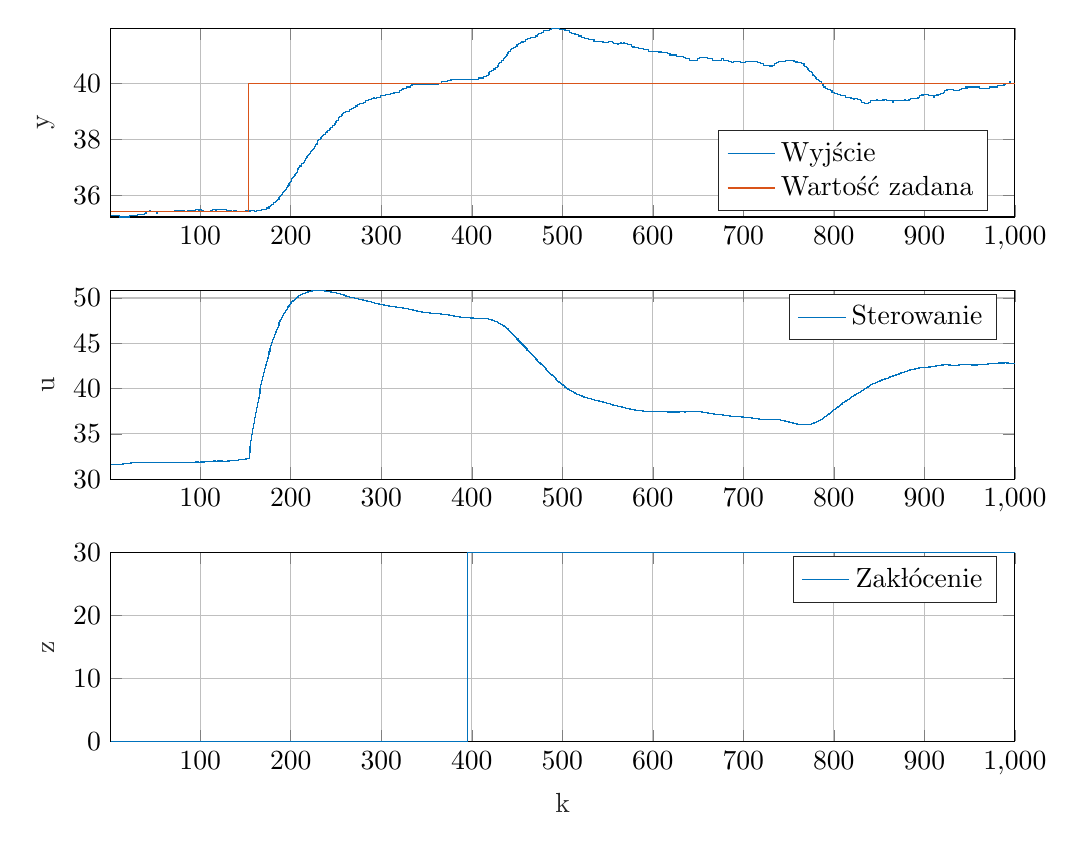
\begin{tikzpicture}

\begin{axis}[%
width=4.521in,
height=0.944in,
at={(0.758in,1.792in)},
scale only axis,
xmin=1,
xmax=1000,
ymin=30,
ymax=50.842440570523,
ylabel style={font=\color{white!15!black}},
ylabel={u},
axis background/.style={fill=white},
xmajorgrids,
ymajorgrids,
legend style={legend cell align=left, align=left, draw=white!15!black}
]
\addplot[const plot, color=mycolor1] table[row sep=crcr] {%
1	31.6478288431062\\
2	31.6456418383518\\
3	31.6441838351822\\
4	31.6434548335975\\
5	31.6434548335975\\
6	31.6441838351822\\
7	31.644912836767\\
8	31.6470998415214\\
9	31.6492868462757\\
10	31.6522028526149\\
11	31.6558478605388\\
12	31.6594928684628\\
13	31.6704278922345\\
14	31.6813629160063\\
15	31.6922979397781\\
16	31.7039619651347\\
17	31.7156259904913\\
18	31.7272900158479\\
19	31.7396830427892\\
20	31.7520760697306\\
21	31.7644690966719\\
22	31.7768621236133\\
23	31.7899841521395\\
24	31.7965451664025\\
25	31.8031061806656\\
26	31.8103961965135\\
27	31.8176862123613\\
28	31.8249762282092\\
29	31.8329952456418\\
30	31.8410142630745\\
31	31.8490332805071\\
32	31.8577812995246\\
33	31.8585103011093\\
34	31.8606973058637\\
35	31.8621553090333\\
36	31.8643423137876\\
37	31.8672583201268\\
38	31.8701743264659\\
39	31.8730903328051\\
40	31.8701743264659\\
41	31.8679873217116\\
42	31.8599683042789\\
43	31.8519492868463\\
44	31.8453882725832\\
45	31.8388272583201\\
46	31.8264342313788\\
47	31.8213312202853\\
48	31.8169572107765\\
49	31.8125832012678\\
50	31.8096671949287\\
51	31.8060221870047\\
52	31.8038351822504\\
53	31.801648177496\\
54	31.8067511885895\\
55	31.80529318542\\
56	31.8045641838352\\
57	31.8038351822504\\
58	31.8038351822504\\
59	31.8045641838352\\
60	31.80529318542\\
61	31.8060221870047\\
62	31.8074801901743\\
63	31.8096671949287\\
64	31.811854199683\\
65	31.8140412044374\\
66	31.8169572107765\\
67	31.8198732171157\\
68	31.8235182250396\\
69	31.8264342313788\\
70	31.8308082408875\\
71	31.8344532488114\\
72	31.8388272583201\\
73	31.8432012678288\\
74	31.8417432646593\\
75	31.8402852614897\\
76	31.8395562599049\\
77	31.8388272583201\\
78	31.8388272583201\\
79	31.8388272583201\\
80	31.8395562599049\\
81	31.8402852614897\\
82	31.8410142630745\\
83	31.8424722662441\\
84	31.8512202852615\\
85	31.8592393026941\\
86	31.8672583201268\\
87	31.8760063391442\\
88	31.8774643423138\\
89	31.8796513470681\\
90	31.8825673534073\\
91	31.8847543581616\\
92	31.8876703645008\\
93	31.8905863708399\\
94	31.8942313787639\\
95	31.897147385103\\
96	31.9007923930269\\
97	31.897147385103\\
98	31.8942313787639\\
99	31.8905863708399\\
100	31.8956893819334\\
101	31.8927733755943\\
102	31.8905863708399\\
103	31.8964183835182\\
104	31.9022503961965\\
105	31.9080824088748\\
106	31.9204754358162\\
107	31.9321394611727\\
108	31.9445324881141\\
109	31.9561965134707\\
110	31.968589540412\\
111	31.9802535657686\\
112	31.9919175911252\\
113	31.9970206022187\\
114	32.0021236133122\\
115	32.0079556259905\\
116	32.0057686212361\\
117	32.0043106180666\\
118	32.0021236133122\\
119	32.0086846275753\\
120	32.0072266244057\\
121	32.0064976228209\\
122	32.0050396196513\\
123	32.0050396196513\\
124	32.0043106180666\\
125	32.0035816164818\\
126	32.0035816164818\\
127	32.0035816164818\\
128	32.0043106180666\\
129	32.0043106180666\\
130	32.0050396196513\\
131	32.013058637084\\
132	32.0210776545166\\
133	32.0290966719493\\
134	32.0371156893819\\
135	32.0516957210776\\
136	32.0597147385103\\
137	32.0735657686212\\
138	32.0874167987322\\
139	32.09470681458\\
140	32.108557844691\\
141	32.115118858954\\
142	32.128969889065\\
143	32.1420919175911\\
144	32.1544849445325\\
145	32.1676069730586\\
146	32.18\\
147	32.1916640253566\\
148	32.2040570522979\\
149	32.2157210776545\\
150	32.2273851030111\\
151	32.2390491283677\\
152	32.2390491283677\\
153	32.2390491283677\\
154	32.9418066561014\\
155	33.624881141046\\
156	34.2948335974643\\
157	34.9458320126783\\
158	35.5713153724247\\
159	36.1785736925515\\
160	36.7676069730586\\
161	37.3398732171157\\
162	37.9019334389857\\
163	38.4472266244057\\
164	38.9699207606973\\
165	39.4765768621236\\
166	39.9686529318542\\
167	40.4461489698891\\
168	40.9090649762282\\
169	41.3581299524564\\
170	41.7882408874802\\
171	42.2052297939778\\
172	42.6098256735341\\
173	43.0027575277337\\
174	43.3840253565769\\
175	43.7477971473851\\
176	44.1013629160063\\
177	44.4454516640254\\
178	44.7742313787639\\
179	45.0949920760697\\
180	45.4011727416799\\
181	45.6927733755943\\
182	45.9785419968304\\
183	46.2497305863708\\
184	46.515087163233\\
185	46.7680507131537\\
186	47.0093502377179\\
187	47.2397147385103\\
188	47.4649762282092\\
189	47.6785736925515\\
190	47.8834231378764\\
191	48.0780665610143\\
192	48.2639619651347\\
193	48.4403803486529\\
194	48.6080507131537\\
195	48.7684310618067\\
196	48.9200633914421\\
197	49.0644057052298\\
198	49.2007290015848\\
199	49.3304912836767\\
200	49.4536925515055\\
201	49.5696038034865\\
202	49.6789540412044\\
203	49.7766402535658\\
204	49.867765451664\\
205	49.9545166402536\\
206	50.0361648177496\\
207	50.1127099841521\\
208	50.1841521394612\\
209	50.2453882725832\\
210	50.3022503961965\\
211	50.3547385103011\\
212	50.4043106180666\\
213	50.4567987321712\\
214	50.4990808240887\\
215	50.5450079239303\\
216	50.5872900158479\\
217	50.6259270998415\\
218	50.6558161648178\\
219	50.68206022187\\
220	50.7053882725832\\
221	50.7330903328051\\
222	50.757147385103\\
223	50.7790174326466\\
224	50.7972424722662\\
225	50.8125515055468\\
226	50.8256735340729\\
227	50.8358795562599\\
228	50.842440570523\\
229	50.8402535657686\\
230	50.842440570523\\
231	50.842440570523\\
232	50.8329635499208\\
233	50.8205705229794\\
234	50.8125515055468\\
235	50.8023454833597\\
236	50.7892234548336\\
237	50.7731854199683\\
238	50.7549603803486\\
239	50.7418383518225\\
240	50.7258003169572\\
241	50.7148652931854\\
242	50.7002852614897\\
243	50.6827892234548\\
244	50.6703961965135\\
245	50.6558161648178\\
246	50.6390491283677\\
247	50.6266561014263\\
248	50.6040570522979\\
249	50.5865610142631\\
250	50.5661489698891\\
251	50.5435499207607\\
252	50.5180348652932\\
253	50.4903328050713\\
254	50.4670047543582\\
255	50.4349286846276\\
256	50.3999366085578\\
257	50.368589540412\\
258	50.3357844690967\\
259	50.3007923930269\\
260	50.2636133122028\\
261	50.2308082408875\\
262	50.1936291600634\\
263	50.1615530903328\\
264	50.1316640253566\\
265	50.1068779714738\\
266	50.0850079239303\\
267	50.0602218700475\\
268	50.038351822504\\
269	50.0128367670364\\
270	49.9909667194929\\
271	49.9654516640254\\
272	49.9435816164818\\
273	49.9238985736925\\
274	49.9005705229794\\
275	49.8794294770206\\
276	49.8546434231379\\
277	49.8320443740095\\
278	49.806529318542\\
279	49.7824722662441\\
280	49.7606022187005\\
281	49.7409191759112\\
282	49.7161331220285\\
283	49.6942630744849\\
284	49.6738510301109\\
285	49.6483359746434\\
286	49.6242789223455\\
287	49.6016798732171\\
288	49.57470681458\\
289	49.5484627575277\\
290	49.5244057052298\\
291	49.4952456418384\\
292	49.4682725832013\\
293	49.4427575277337\\
294	49.4128684627575\\
295	49.3909984152139\\
296	49.3705863708399\\
297	49.3450713153724\\
298	49.322472266244\\
299	49.3006022187005\\
300	49.2809191759113\\
301	49.2561331220285\\
302	49.2335340729002\\
303	49.2123930269414\\
304	49.1934389857369\\
305	49.1766719492868\\
306	49.1620919175911\\
307	49.1438668779715\\
308	49.1263708399366\\
309	49.1117908082409\\
310	49.0979397781299\\
311	49.0862757527734\\
312	49.0695087163233\\
313	49.0541996830428\\
314	49.0403486529318\\
315	49.0286846275753\\
316	49.0111885895404\\
317	48.9958795562599\\
318	48.982028526149\\
319	48.9696354992076\\
320	48.9587004754358\\
321	48.9484944532488\\
322	48.9324564183835\\
323	48.917147385103\\
324	48.8974643423138\\
325	48.8792393026941\\
326	48.855911251981\\
327	48.8347702060222\\
328	48.815087163233\\
329	48.7961331220285\\
330	48.7728050713154\\
331	48.7509350237718\\
332	48.7312519809826\\
333	48.7130269413629\\
334	48.688969889065\\
335	48.6656418383518\\
336	48.6386687797147\\
337	48.6131537242472\\
338	48.5883676703645\\
339	48.5657686212361\\
340	48.5446275752773\\
341	48.5242155309033\\
342	48.5045324881141\\
343	48.4863074484944\\
344	48.4695404120444\\
345	48.4527733755943\\
346	48.436735340729\\
347	48.4214263074485\\
348	48.4068462757528\\
349	48.3929952456418\\
350	48.3798732171157\\
351	48.3674801901743\\
352	48.3558161648177\\
353	48.3456101426307\\
354	48.3354041204437\\
355	48.3259270998415\\
356	48.3171790808241\\
357	48.3084310618067\\
358	48.300412044374\\
359	48.2931220285261\\
360	48.2851030110935\\
361	48.2778129952456\\
362	48.2712519809826\\
363	48.2646909667195\\
364	48.2588589540412\\
365	48.2471949286846\\
366	48.2362599049128\\
367	48.2260538827258\\
368	48.2158478605388\\
369	48.2005388272583\\
370	48.1852297939778\\
371	48.1713787638669\\
372	48.1567987321712\\
373	48.1444057052298\\
374	48.1312836767036\\
375	48.1123296354992\\
376	48.0941045958796\\
377	48.0773375594295\\
378	48.0612995245642\\
379	48.0401584786054\\
380	48.0197464342314\\
381	48.0007923930269\\
382	47.9825673534073\\
383	47.966529318542\\
384	47.9504912836767\\
385	47.9351822503962\\
386	47.9206022187005\\
387	47.9074801901743\\
388	47.895087163233\\
389	47.8841521394612\\
390	47.8732171156894\\
391	47.8630110935024\\
392	47.8535340729002\\
393	47.8440570522979\\
394	47.8360380348653\\
395	47.8287480190174\\
396	47.8214580031696\\
397	47.8141679873217\\
398	47.8083359746434\\
399	47.8017749603803\\
400	47.7959429477021\\
401	47.7908399366085\\
402	47.7864659270998\\
403	47.7820919175911\\
404	47.7784469096672\\
405	47.775530903328\\
406	47.7733438985737\\
407	47.7711568938193\\
408	47.7696988906498\\
409	47.7616798732171\\
410	47.7543898573693\\
411	47.7478288431062\\
412	47.7412678288431\\
413	47.73470681458\\
414	47.7288748019017\\
415	47.7172107765452\\
416	47.7055467511886\\
417	47.693882725832\\
418	47.6756576862124\\
419	47.6581616481775\\
420	47.6355625990491\\
421	47.6064025356577\\
422	47.571410459588\\
423	47.537147385103\\
424	47.4977812995246\\
425	47.4584152139461\\
426	47.414675118859\\
427	47.3723930269414\\
428	47.3250079239303\\
429	47.2798098256735\\
430	47.2287797147385\\
431	47.17264659271\\
432	47.1121394611727\\
433	47.046529318542\\
434	46.9838351822504\\
435	46.9080190174326\\
436	46.835118858954\\
437	46.7585736925515\\
438	46.6769255150555\\
439	46.5916323296355\\
440	46.501236133122\\
441	46.4071949286846\\
442	46.3087797147385\\
443	46.2074484944532\\
444	46.1090332805071\\
445	46.0055150554675\\
446	45.898351822504\\
447	45.7941045958796\\
448	45.6862123613312\\
449	45.581236133122\\
450	45.4726148969889\\
451	45.3669096671949\\
452	45.2568304278922\\
453	45.1489381933439\\
454	45.0374009508716\\
455	44.9287797147385\\
456	44.8172424722662\\
457	44.70206022187\\
458	44.5963549920761\\
459	44.4870047543582\\
460	44.3798415213946\\
461	44.2690332805071\\
462	44.1611410459588\\
463	44.0561648177496\\
464	43.9475435816165\\
465	43.8418383518225\\
466	43.7390491283677\\
467	43.6318858954041\\
468	43.5276386687797\\
469	43.4255784469097\\
470	43.3264342313788\\
471	43.2287480190174\\
472	43.1274167987322\\
473	43.0282725832013\\
474	42.9305863708399\\
475	42.8277971473851\\
476	42.7220919175911\\
477	42.6185736925515\\
478	42.517971473851\\
479	42.4129952456418\\
480	42.3109350237718\\
481	42.2037717908082\\
482	42.098795562599\\
483	41.996735340729\\
484	41.8961331220285\\
485	41.7984469096672\\
486	41.7014896988906\\
487	41.6067194928685\\
488	41.5068462757528\\
489	41.4091600633914\\
490	41.3070998415214\\
491	41.2072266244057\\
492	41.1088114104596\\
493	41.0125832012678\\
494	40.9185419968304\\
495	40.8259587955626\\
496	40.7348335974643\\
497	40.6458954041204\\
498	40.5576862123613\\
499	40.4774960380349\\
500	40.398763866878\\
501	40.3207606973059\\
502	40.2442155309033\\
503	40.1683993660856\\
504	40.0933122028526\\
505	40.0262440570523\\
506	39.9606339144215\\
507	39.8950237717908\\
508	39.8301426307448\\
509	39.7652614896989\\
510	39.7076703645008\\
511	39.6500792393027\\
512	39.5983201267829\\
513	39.5472900158479\\
514	39.4962599049128\\
515	39.4452297939778\\
516	39.4000316957211\\
517	39.3541045958795\\
518	39.3096354992076\\
519	39.2637083993661\\
520	39.2258003169572\\
521	39.1864342313788\\
522	39.1470681458003\\
523	39.1135340729002\\
524	39.0785419968304\\
525	39.0442789223455\\
526	39.0092868462757\\
527	38.9808557844691\\
528	38.9516957210776\\
529	38.9210776545166\\
530	38.8897305863708\\
531	38.8634865293185\\
532	38.8365134706815\\
533	38.8088114104596\\
534	38.7803803486529\\
535	38.7512202852615\\
536	38.72206022187\\
537	38.6994611727417\\
538	38.6768621236133\\
539	38.6535340729002\\
540	38.6287480190174\\
541	38.6032329635499\\
542	38.5777179080824\\
543	38.5507448494453\\
544	38.5230427892235\\
545	38.4953407290016\\
546	38.4669096671949\\
547	38.4450396196513\\
548	38.4217115689382\\
549	38.398383518225\\
550	38.3743264659271\\
551	38.3495404120444\\
552	38.3247543581616\\
553	38.2926782884311\\
554	38.2606022187005\\
555	38.2277971473851\\
556	38.1949920760697\\
557	38.1680190174326\\
558	38.1410459587956\\
559	38.1199049128368\\
560	38.0980348652932\\
561	38.0761648177496\\
562	38.0535657686212\\
563	38.0360697305864\\
564	38.0120126782884\\
565	37.9879556259905\\
566	37.9566085578447\\
567	37.931822503962\\
568	37.9063074484945\\
569	37.8800633914421\\
570	37.8479873217116\\
571	37.8210142630745\\
572	37.7947702060222\\
573	37.7670681458003\\
574	37.7459270998415\\
575	37.7247860538827\\
576	37.7021870047544\\
577	37.679587955626\\
578	37.6642789223455\\
579	37.6475118858954\\
580	37.6373058637084\\
581	37.6190808240887\\
582	37.6074167987322\\
583	37.594294770206\\
584	37.5819017432647\\
585	37.5680507131537\\
586	37.5600316957211\\
587	37.5520126782884\\
588	37.5425356576862\\
589	37.533058637084\\
590	37.522852614897\\
591	37.51264659271\\
592	37.5075435816165\\
593	37.502440570523\\
594	37.4973375594295\\
595	37.4907765451664\\
596	37.4842155309033\\
597	37.4849445324881\\
598	37.4849445324881\\
599	37.4842155309033\\
600	37.4827575277338\\
601	37.4805705229794\\
602	37.4776545166402\\
603	37.4740095087163\\
604	37.4703645007924\\
605	37.4659904912837\\
606	37.4608874801902\\
607	37.4550554675119\\
608	37.4557844690967\\
609	37.4484944532488\\
610	37.4412044374009\\
611	37.4397464342314\\
612	37.437559429477\\
613	37.4346434231379\\
614	37.4309984152139\\
615	37.42735340729\\
616	37.4229793977813\\
617	37.417147385103\\
618	37.417147385103\\
619	37.4156893819334\\
620	37.4135023771791\\
621	37.417147385103\\
622	37.4193343898574\\
623	37.4207923930269\\
624	37.4222503961965\\
625	37.4222503961965\\
626	37.4222503961965\\
627	37.4207923930269\\
628	37.4251664025357\\
629	37.4280824088748\\
630	37.4302694136292\\
631	37.4317274167987\\
632	37.4317274167987\\
633	37.4302694136292\\
634	37.42735340729\\
635	37.4244374009509\\
636	37.4258954041204\\
637	37.4266244057052\\
638	37.4324564183835\\
639	37.4368304278922\\
640	37.4397464342314\\
641	37.4419334389857\\
642	37.4426624405705\\
643	37.4492234548336\\
644	37.4535974643423\\
645	37.4572424722662\\
646	37.4601584786054\\
647	37.461616481775\\
648	37.4623454833597\\
649	37.461616481775\\
650	37.4601584786054\\
651	37.451410459588\\
652	37.4419334389857\\
653	37.4317274167987\\
654	37.4142313787639\\
655	37.396735340729\\
656	37.3792393026941\\
657	37.3610142630745\\
658	37.34206022187\\
659	37.3231061806656\\
660	37.3041521394612\\
661	37.2844690966719\\
662	37.2713470681458\\
663	37.2574960380349\\
664	37.2436450079239\\
665	37.2290649762282\\
666	37.2144849445325\\
667	37.199175911252\\
668	37.1904278922345\\
669	37.1809508716323\\
670	37.1707448494453\\
671	37.1605388272583\\
672	37.1503328050713\\
673	37.1393977812995\\
674	37.1277337559429\\
675	37.1160697305864\\
676	37.1044057052298\\
677	37.0920126782884\\
678	37.073058637084\\
679	37.0541045958796\\
680	37.0409825673534\\
681	37.028589540412\\
682	37.0154675118859\\
683	37.001616481775\\
684	36.9884944532488\\
685	36.9746434231379\\
686	36.9680824088748\\
687	36.9607923930269\\
688	36.9535023771791\\
689	36.9520443740095\\
690	36.9505863708399\\
691	36.9418383518225\\
692	36.9323613312203\\
693	36.9228843106181\\
694	36.9134072900158\\
695	36.9032012678288\\
696	36.8929952456418\\
697	36.88206022187\\
698	36.8711251980983\\
699	36.8667511885895\\
700	36.861648177496\\
701	36.8558161648177\\
702	36.8499841521395\\
703	36.8434231378764\\
704	36.8303011093502\\
705	36.8171790808241\\
706	36.8033280507132\\
707	36.790206022187\\
708	36.7763549920761\\
709	36.7625039619651\\
710	36.7479239302694\\
711	36.7340729001585\\
712	36.7194928684628\\
713	36.704912836767\\
714	36.6903328050713\\
715	36.6757527733756\\
716	36.6611727416799\\
717	36.6458637083994\\
718	36.6371156893819\\
719	36.6283676703645\\
720	36.6188906497623\\
721	36.6159746434231\\
722	36.613058637084\\
723	36.6086846275753\\
724	36.6108716323296\\
725	36.613058637084\\
726	36.6137876386688\\
727	36.6145166402536\\
728	36.6145166402536\\
729	36.6145166402536\\
730	36.6137876386688\\
731	36.6203486529319\\
732	36.6181616481775\\
733	36.623264659271\\
734	36.6203486529319\\
735	36.6174326465927\\
736	36.6072266244057\\
737	36.5970206022187\\
738	36.5868145800317\\
739	36.5707765451664\\
740	36.5540095087163\\
741	36.5306814580032\\
742	36.5080824088748\\
743	36.4854833597464\\
744	36.4628843106181\\
745	36.4410142630745\\
746	36.4191442155309\\
747	36.3972741679873\\
748	36.3761331220285\\
749	36.3477020602219\\
750	36.3192709984152\\
751	36.2915689381933\\
752	36.2638668779715\\
753	36.2368938193344\\
754	36.2106497622821\\
755	36.1844057052298\\
756	36.1581616481775\\
757	36.13264659271\\
758	36.1151505546751\\
759	36.0976545166402\\
760	36.0859904912837\\
761	36.0684944532488\\
762	36.057559429477\\
763	36.0458954041204\\
764	36.0349603803487\\
765	36.0232963549921\\
766	36.0181933438986\\
767	36.0123613312203\\
768	36.006529318542\\
769	36.0072583201268\\
770	36.0145483359746\\
771	36.0211093502377\\
772	36.0335023771791\\
773	36.0509984152139\\
774	36.0743264659271\\
775	36.1042155309033\\
776	36.13264659271\\
777	36.1654516640254\\
778	36.204088748019\\
779	36.2470998415214\\
780	36.2886529318542\\
781	36.3353090332805\\
782	36.3870681458003\\
783	36.4432012678288\\
784	36.497147385103\\
785	36.5554675118859\\
786	36.6188906497623\\
787	36.6801267828843\\
788	36.7457369255151\\
789	36.8149920760697\\
790	36.8878922345483\\
791	36.9666244057052\\
792	37.0417115689382\\
793	37.1211727416799\\
794	37.1969889064976\\
795	37.2771790808241\\
796	37.3544532488114\\
797	37.4295404120444\\
798	37.5075435816165\\
799	37.5833597464342\\
800	37.6642789223455\\
801	37.7422820919176\\
802	37.8173692551506\\
803	37.8961014263074\\
804	37.97264659271\\
805	38.0470047543582\\
806	38.1242789223455\\
807	38.2000950871632\\
808	38.2729952456418\\
809	38.3495404120444\\
810	38.4246275752773\\
811	38.4967987321712\\
812	38.5667828843106\\
813	38.6345800316957\\
814	38.7001901743265\\
815	38.7716323296355\\
816	38.8408874801902\\
817	38.9079556259905\\
818	38.9728367670364\\
819	39.0362599049128\\
820	39.0974960380349\\
821	39.1638351822504\\
822	39.2287163232964\\
823	39.291410459588\\
824	39.3584786053883\\
825	39.4182567353407\\
826	39.4758478605388\\
827	39.5319809825673\\
828	39.5939461172742\\
829	39.6537242472266\\
830	39.7120443740095\\
831	39.7754675118859\\
832	39.8374326465927\\
833	39.9052297939778\\
834	39.9715689381933\\
835	40.0364500792393\\
836	40.1064342313788\\
837	40.1742313787639\\
838	40.2412995245642\\
839	40.3069096671949\\
840	40.364500792393\\
841	40.4206339144216\\
842	40.4760380348653\\
843	40.5226941362916\\
844	40.5686212361331\\
845	40.6145483359746\\
846	40.6590174326466\\
847	40.7027575277338\\
848	40.7464976228209\\
849	40.7829477020602\\
850	40.8252297939778\\
851	40.8667828843106\\
852	40.9083359746434\\
853	40.9484310618067\\
854	40.9892551505547\\
855	41.0286212361331\\
856	41.0614263074485\\
857	41.1007923930269\\
858	41.1335974643423\\
859	41.1656735340729\\
860	41.2035816164818\\
861	41.2422187004754\\
862	41.2793977812995\\
863	41.3173058637084\\
864	41.3544849445325\\
865	41.3916640253566\\
866	41.4281141045959\\
867	41.471854199683\\
868	41.5075752773376\\
869	41.5440253565769\\
870	41.5790174326466\\
871	41.6147385103011\\
872	41.6504595879556\\
873	41.6854516640254\\
874	41.7204437400951\\
875	41.75470681458\\
876	41.7896988906498\\
877	41.8239619651347\\
878	41.8582250396196\\
879	41.8924881141046\\
880	41.9201901743265\\
881	41.9537242472266\\
882	41.9879873217116\\
883	42.0215213946117\\
884	42.0550554675119\\
885	42.082028526149\\
886	42.1097305863708\\
887	42.1301426307448\\
888	42.1512836767036\\
889	42.1724247226624\\
890	42.194294770206\\
891	42.2161648177496\\
892	42.2380348652932\\
893	42.2599049128368\\
894	42.2825039619651\\
895	42.2985419968304\\
896	42.3153090332805\\
897	42.3247860538827\\
898	42.3342630744849\\
899	42.3386370839937\\
900	42.3503011093502\\
901	42.3554041204437\\
902	42.3619651347068\\
903	42.3685261489699\\
904	42.3758161648177\\
905	42.3838351822504\\
906	42.391854199683\\
907	42.4078922345483\\
908	42.4232012678288\\
909	42.4399683042789\\
910	42.4560063391442\\
911	42.4727733755943\\
912	42.497559429477\\
913	42.5150554675119\\
914	42.5325515055467\\
915	42.5500475435816\\
916	42.5617115689382\\
917	42.5799366085578\\
918	42.5923296354992\\
919	42.6054516640254\\
920	42.6120126782884\\
921	42.6193026941363\\
922	42.6273217115689\\
923	42.6295087163233\\
924	42.6251347068146\\
925	42.6214896988906\\
926	42.6185736925515\\
927	42.6098256735341\\
928	42.6025356576862\\
929	42.5967036450079\\
930	42.5908716323296\\
931	42.5864976228209\\
932	42.582852614897\\
933	42.5799366085578\\
934	42.5850396196513\\
935	42.5901426307448\\
936	42.5959746434231\\
937	42.6018066561014\\
938	42.6090966719493\\
939	42.6163866877971\\
940	42.6251347068146\\
941	42.6273217115689\\
942	42.6302377179081\\
943	42.6273217115689\\
944	42.6258637083994\\
945	42.6244057052298\\
946	42.6244057052298\\
947	42.6244057052298\\
948	42.6193026941363\\
949	42.6207606973059\\
950	42.6171156893819\\
951	42.6141996830428\\
952	42.6120126782884\\
953	42.6105546751189\\
954	42.6098256735341\\
955	42.6098256735341\\
956	42.6105546751189\\
957	42.6112836767036\\
958	42.613470681458\\
959	42.6156576862124\\
960	42.6185736925515\\
961	42.6222187004754\\
962	42.6258637083994\\
963	42.6367987321712\\
964	42.6477337559429\\
965	42.6586687797147\\
966	42.6703328050713\\
967	42.6819968304279\\
968	42.6936608557845\\
969	42.7060538827258\\
970	42.7184469096672\\
971	42.7308399366086\\
972	42.7432329635499\\
973	42.7563549920761\\
974	42.7629160063391\\
975	42.7694770206022\\
976	42.7767670364501\\
977	42.7840570522979\\
978	42.7913470681458\\
979	42.7993660855784\\
980	42.8073851030111\\
981	42.8154041204437\\
982	42.8241521394612\\
983	42.824881141046\\
984	42.8270681458003\\
985	42.8285261489699\\
986	42.8307131537242\\
987	42.8336291600634\\
988	42.8365451664025\\
989	42.8394611727417\\
990	42.8365451664025\\
991	42.8343581616482\\
992	42.8263391442155\\
993	42.8183201267829\\
994	42.8117591125198\\
995	42.8051980982567\\
996	42.7928050713154\\
997	42.7877020602219\\
998	42.7833280507132\\
999	42.7789540412044\\
1000	42.7760380348653\\
1001	42.7723930269414\\
1002	42.770206022187\\
1003	42.7680190174326\\
1004	42.7731220285261\\
1005	42.7716640253566\\
1006	42.7709350237718\\
1007	42.770206022187\\
1008	42.770206022187\\
1009	42.7709350237718\\
1010	42.7716640253566\\
1011	42.7723930269414\\
1012	42.7738510301109\\
1013	42.7760380348653\\
1014	42.7782250396196\\
1015	42.780412044374\\
1016	42.7833280507132\\
1017	42.7862440570523\\
1018	42.7898890649762\\
1019	42.7928050713154\\
1020	42.7971790808241\\
1021	42.800824088748\\
1022	42.8051980982567\\
1023	42.8095721077654\\
1024	42.8081141045959\\
1025	42.8066561014263\\
1026	42.8059270998415\\
1027	42.8051980982567\\
1028	42.8051980982567\\
1029	42.8051980982567\\
1030	42.8059270998415\\
1031	42.8066561014263\\
1032	42.8073851030111\\
1033	42.8088431061807\\
1034	42.8175911251981\\
1035	42.8256101426307\\
1036	42.8336291600634\\
1037	42.8423771790808\\
1038	42.8438351822504\\
1039	42.8460221870047\\
1040	42.8489381933439\\
1041	42.8511251980983\\
1042	42.8540412044374\\
1043	42.8569572107765\\
1044	42.8606022187005\\
1045	42.8635182250396\\
1046	42.8671632329635\\
1047	42.8635182250396\\
1048	42.8606022187005\\
1049	42.8569572107765\\
1050	42.86206022187\\
1051	42.8591442155309\\
1052	42.8569572107765\\
1053	42.8627892234548\\
1054	42.8686212361331\\
1055	42.8744532488114\\
1056	42.8868462757528\\
1057	42.8985103011093\\
1058	42.9109033280507\\
1059	42.9225673534073\\
1060	42.9349603803486\\
1061	42.9466244057052\\
1062	42.9582884310618\\
1063	42.9633914421553\\
1064	42.9684944532488\\
1065	42.9743264659271\\
1066	42.9721394611727\\
1067	42.9706814580032\\
1068	42.9684944532488\\
1069	42.9750554675119\\
1070	42.9735974643423\\
1071	42.9728684627575\\
1072	42.971410459588\\
1073	42.971410459588\\
1074	42.9706814580032\\
1075	42.9699524564184\\
1076	42.9699524564184\\
1077	42.9699524564184\\
1078	42.9706814580032\\
1079	42.9706814580032\\
1080	42.971410459588\\
1081	42.9794294770206\\
1082	42.9874484944532\\
1083	42.9954675118859\\
1084	43.0034865293185\\
1085	43.0180665610143\\
1086	43.0260855784469\\
1087	43.0399366085578\\
1088	43.0537876386688\\
1089	43.0610776545166\\
1090	43.0749286846276\\
1091	43.0814896988906\\
1092	43.0953407290016\\
1093	43.1084627575277\\
1094	43.1208557844691\\
1095	43.1339778129952\\
1096	43.1463708399366\\
1097	43.1580348652932\\
1098	43.1704278922345\\
1099	43.1820919175911\\
1100	43.1937559429477\\
1101	43.2054199683043\\
1102	43.209793977813\\
1103	43.2148969889065\\
1104	43.22\\
1105	43.2251030110935\\
1106	43.230206022187\\
1107	43.2418700475436\\
1108	43.2462440570523\\
1109	43.2513470681458\\
1110	43.2564500792393\\
1111	43.2622820919176\\
1112	43.2673851030111\\
1113	43.2724881141046\\
1114	43.2783201267829\\
1115	43.2834231378764\\
1116	43.2892551505547\\
1117	43.301648177496\\
1118	43.3133122028526\\
1119	43.3249762282092\\
1120	43.3373692551505\\
1121	43.3490332805071\\
1122	43.366529318542\\
1123	43.3840253565769\\
1124	43.4015213946117\\
1125	43.4190174326466\\
1126	43.4357844690967\\
1127	43.451822503962\\
1128	43.468589540412\\
1129	43.4846275752773\\
1130	43.4999366085578\\
1131	43.5159746434231\\
1132	43.5378446909667\\
1133	43.5589857369255\\
1134	43.5801267828843\\
1135	43.5939778129952\\
1136	43.6078288431062\\
1137	43.6216798732171\\
1138	43.635530903328\\
1139	43.6552139461173\\
1140	43.6683359746434\\
1141	43.6814580031696\\
1142	43.6880190174326\\
1143	43.6945800316957\\
1144	43.6945800316957\\
1145	43.6953090332805\\
1146	43.6960380348653\\
1147	43.6894770206022\\
1148	43.6770839936609\\
1149	43.6654199683043\\
1150	43.6544849445325\\
1151	43.6369889064976\\
};
\addlegendentry{Sterowanie}

\end{axis}

\begin{axis}[%
width=4.521in,
height=0.944in,
at={(0.758in,3.103in)},
scale only axis,
xmin=1,
xmax=1000,
ymin=35.2177496038035,
ymax=41.9610142630745,
ylabel style={font=\color{white!15!black}},
ylabel={y},
axis background/.style={fill=white},
xmajorgrids,
ymajorgrids,
legend style={at={(0.97,0.03)}, anchor=south east, legend cell align=left, align=left, draw=white!15!black}
]
\addplot[const plot, color=mycolor1] table[row sep=crcr] {%
1	35.2614896988906\\
2	35.2614896988906\\
3	35.2614896988906\\
4	35.2614896988906\\
5	35.2614896988906\\
6	35.2614896988906\\
7	35.2614896988906\\
8	35.2614896988906\\
9	35.2614896988906\\
10	35.2614896988906\\
11	35.2177496038035\\
12	35.2177496038035\\
13	35.2177496038035\\
14	35.2177496038035\\
15	35.2177496038035\\
16	35.2177496038035\\
17	35.2177496038035\\
18	35.2177496038035\\
19	35.2177496038035\\
20	35.2177496038035\\
21	35.2177496038035\\
22	35.2614896988906\\
23	35.2614896988906\\
24	35.2614896988906\\
25	35.2614896988906\\
26	35.2614896988906\\
27	35.2614896988906\\
28	35.2614896988906\\
29	35.2614896988906\\
30	35.2614896988906\\
31	35.3125198098257\\
32	35.3125198098257\\
33	35.3125198098257\\
34	35.3125198098257\\
35	35.3125198098257\\
36	35.3125198098257\\
37	35.3125198098257\\
38	35.3562599049128\\
39	35.3562599049128\\
40	35.4\\
41	35.4\\
42	35.4\\
43	35.4\\
44	35.4437400950872\\
45	35.4\\
46	35.4\\
47	35.4\\
48	35.4\\
49	35.4\\
50	35.4\\
51	35.4\\
52	35.3562599049128\\
53	35.4\\
54	35.4\\
55	35.4\\
56	35.4\\
57	35.4\\
58	35.4\\
59	35.4\\
60	35.4\\
61	35.4\\
62	35.4\\
63	35.4\\
64	35.4\\
65	35.4\\
66	35.4\\
67	35.4\\
68	35.4\\
69	35.4\\
70	35.4\\
71	35.4\\
72	35.4437400950872\\
73	35.4437400950872\\
74	35.4437400950872\\
75	35.4437400950872\\
76	35.4437400950872\\
77	35.4437400950872\\
78	35.4437400950872\\
79	35.4437400950872\\
80	35.4437400950872\\
81	35.4437400950872\\
82	35.4\\
83	35.4\\
84	35.4\\
85	35.4\\
86	35.4437400950872\\
87	35.4437400950872\\
88	35.4437400950872\\
89	35.4437400950872\\
90	35.4437400950872\\
91	35.4437400950872\\
92	35.4437400950872\\
93	35.4437400950872\\
94	35.4437400950872\\
95	35.4947702060222\\
96	35.4947702060222\\
97	35.4947702060222\\
98	35.4437400950872\\
99	35.4947702060222\\
100	35.4947702060222\\
101	35.4437400950872\\
102	35.4437400950872\\
103	35.4437400950872\\
104	35.4\\
105	35.4\\
106	35.4\\
107	35.4\\
108	35.4\\
109	35.4\\
110	35.4\\
111	35.4437400950872\\
112	35.4437400950872\\
113	35.4437400950872\\
114	35.4947702060222\\
115	35.4947702060222\\
116	35.4947702060222\\
117	35.4437400950872\\
118	35.4947702060222\\
119	35.4947702060222\\
120	35.4947702060222\\
121	35.4947702060222\\
122	35.4947702060222\\
123	35.4947702060222\\
124	35.4947702060222\\
125	35.4947702060222\\
126	35.4947702060222\\
127	35.4947702060222\\
128	35.4947702060222\\
129	35.4437400950872\\
130	35.4437400950872\\
131	35.4437400950872\\
132	35.4437400950872\\
133	35.4\\
134	35.4437400950872\\
135	35.4\\
136	35.4\\
137	35.4437400950872\\
138	35.4\\
139	35.4437400950872\\
140	35.4\\
141	35.4\\
142	35.4\\
143	35.4\\
144	35.4\\
145	35.4\\
146	35.4\\
147	35.4\\
148	35.4\\
149	35.4\\
150	35.4437400950872\\
151	35.4437400950872\\
152	35.4437400950872\\
153	35.4437400950872\\
154	35.4\\
155	35.4\\
156	35.4437400950872\\
157	35.4437400950872\\
158	35.4437400950872\\
159	35.4437400950872\\
160	35.4\\
161	35.4\\
162	35.4437400950872\\
163	35.4437400950872\\
164	35.4437400950872\\
165	35.4437400950872\\
166	35.4437400950872\\
167	35.4437400950872\\
168	35.4874801901743\\
169	35.4874801901743\\
170	35.4874801901743\\
171	35.4874801901743\\
172	35.4874801901743\\
173	35.5385103011094\\
174	35.5385103011094\\
175	35.5385103011094\\
176	35.5822503961965\\
177	35.5822503961965\\
178	35.6259904912837\\
179	35.6697305863708\\
180	35.6697305863708\\
181	35.7207606973059\\
182	35.7207606973059\\
183	35.764500792393\\
184	35.8082408874802\\
185	35.8519809825674\\
186	35.8519809825674\\
187	35.9030110935024\\
188	35.9467511885895\\
189	35.9904912836767\\
190	36.0342313787639\\
191	36.0852614896989\\
192	36.1290015847861\\
193	36.1727416798732\\
194	36.2164817749604\\
195	36.2675118858954\\
196	36.3112519809826\\
197	36.3549920760697\\
198	36.3987321711569\\
199	36.4497622820919\\
200	36.4935023771791\\
201	36.5809825673534\\
202	36.6320126782884\\
203	36.6757527733756\\
204	36.7194928684628\\
205	36.7632329635499\\
206	36.8142630744849\\
207	36.9017432646593\\
208	36.9454833597464\\
209	36.9965134706815\\
210	37.0402535657686\\
211	37.0402535657686\\
212	37.1277337559429\\
213	37.1277337559429\\
214	37.178763866878\\
215	37.2225039619651\\
216	37.3099841521395\\
217	37.3610142630745\\
218	37.4047543581617\\
219	37.4047543581617\\
220	37.4484944532488\\
221	37.492234548336\\
222	37.543264659271\\
223	37.5870047543582\\
224	37.6307448494453\\
225	37.6744849445325\\
226	37.7255150554675\\
227	37.8129952456418\\
228	37.8129952456418\\
229	37.856735340729\\
230	37.9515055467512\\
231	37.9952456418384\\
232	37.9952456418384\\
233	38.0389857369255\\
234	38.0900158478605\\
235	38.1337559429477\\
236	38.1774960380349\\
237	38.1774960380349\\
238	38.221236133122\\
239	38.221236133122\\
240	38.2722662440571\\
241	38.3160063391442\\
242	38.3160063391442\\
243	38.3597464342314\\
244	38.4034865293185\\
245	38.4034865293185\\
246	38.4982567353407\\
247	38.4982567353407\\
248	38.5419968304279\\
249	38.5857369255151\\
250	38.6367670364501\\
251	38.6805071315372\\
252	38.6805071315372\\
253	38.7679873217116\\
254	38.8190174326466\\
255	38.8190174326466\\
256	38.8627575277338\\
257	38.9064976228209\\
258	38.9502377179081\\
259	38.9502377179081\\
260	39.0012678288431\\
261	39.0012678288431\\
262	39.0012678288431\\
263	39.0012678288431\\
264	39.0012678288431\\
265	39.0450079239303\\
266	39.0450079239303\\
267	39.0887480190174\\
268	39.0887480190174\\
269	39.1324881141046\\
270	39.1324881141046\\
271	39.1324881141046\\
272	39.1835182250396\\
273	39.1835182250396\\
274	39.2272583201268\\
275	39.2272583201268\\
276	39.2709984152139\\
277	39.2709984152139\\
278	39.2709984152139\\
279	39.2709984152139\\
280	39.3147385103011\\
281	39.3147385103011\\
282	39.3147385103011\\
283	39.3657686212361\\
284	39.3657686212361\\
285	39.3657686212361\\
286	39.4095087163233\\
287	39.4095087163233\\
288	39.4095087163233\\
289	39.4532488114105\\
290	39.4532488114105\\
291	39.4532488114105\\
292	39.4969889064976\\
293	39.4532488114105\\
294	39.4532488114105\\
295	39.4969889064976\\
296	39.4969889064976\\
297	39.4969889064976\\
298	39.4969889064976\\
299	39.5480190174327\\
300	39.5480190174327\\
301	39.5480190174327\\
302	39.5480190174327\\
303	39.5480190174327\\
304	39.5480190174327\\
305	39.5917591125198\\
306	39.5917591125198\\
307	39.5917591125198\\
308	39.5917591125198\\
309	39.5917591125198\\
310	39.635499207607\\
311	39.635499207607\\
312	39.635499207607\\
313	39.635499207607\\
314	39.6792393026941\\
315	39.6792393026941\\
316	39.6792393026941\\
317	39.6792393026941\\
318	39.6792393026941\\
319	39.6792393026941\\
320	39.7302694136292\\
321	39.7302694136292\\
322	39.7740095087163\\
323	39.7740095087163\\
324	39.8177496038035\\
325	39.8177496038035\\
326	39.8177496038035\\
327	39.8177496038035\\
328	39.8614896988907\\
329	39.8614896988907\\
330	39.8614896988907\\
331	39.8614896988907\\
332	39.9125198098257\\
333	39.9125198098257\\
334	39.9562599049128\\
335	39.9562599049128\\
336	39.9562599049128\\
337	39.9562599049128\\
338	39.9562599049128\\
339	39.9562599049128\\
340	39.9562599049128\\
341	39.9562599049128\\
342	39.9562599049128\\
343	39.9562599049128\\
344	39.9562599049128\\
345	39.9562599049128\\
346	39.9562599049128\\
347	39.9562599049128\\
348	39.9562599049128\\
349	39.9562599049128\\
350	39.9562599049128\\
351	39.9562599049128\\
352	39.9562599049128\\
353	39.9562599049128\\
354	39.9562599049128\\
355	39.9562599049128\\
356	39.9562599049128\\
357	39.9562599049128\\
358	39.9562599049128\\
359	39.9562599049128\\
360	39.9562599049128\\
361	39.9562599049128\\
362	39.9562599049128\\
363	40\\
364	40\\
365	40\\
366	40\\
367	40.0437400950872\\
368	40.0437400950872\\
369	40.0437400950872\\
370	40.0437400950872\\
371	40.0437400950872\\
372	40.0437400950872\\
373	40.0947702060222\\
374	40.0947702060222\\
375	40.0947702060222\\
376	40.0947702060222\\
377	40.1385103011094\\
378	40.1385103011094\\
379	40.1385103011094\\
380	40.1385103011094\\
381	40.1385103011094\\
382	40.1385103011094\\
383	40.1385103011094\\
384	40.1385103011094\\
385	40.1385103011094\\
386	40.1385103011094\\
387	40.1385103011094\\
388	40.1385103011094\\
389	40.1385103011094\\
390	40.1385103011094\\
391	40.1385103011094\\
392	40.1385103011094\\
393	40.1385103011094\\
394	40.1385103011094\\
395	40.1385103011094\\
396	40.1385103011094\\
397	40.1385103011094\\
398	40.1385103011094\\
399	40.1385103011094\\
400	40.1385103011094\\
401	40.1385103011094\\
402	40.1385103011094\\
403	40.1385103011094\\
404	40.1385103011094\\
405	40.1385103011094\\
406	40.1385103011094\\
407	40.1822503961965\\
408	40.1822503961965\\
409	40.1822503961965\\
410	40.1822503961965\\
411	40.1822503961965\\
412	40.1822503961965\\
413	40.2259904912837\\
414	40.2259904912837\\
415	40.2259904912837\\
416	40.2770206022187\\
417	40.2770206022187\\
418	40.3207606973059\\
419	40.364500792393\\
420	40.4082408874802\\
421	40.4082408874802\\
422	40.4592709984152\\
423	40.4592709984152\\
424	40.5030110935024\\
425	40.5030110935024\\
426	40.5467511885895\\
427	40.5467511885895\\
428	40.5904912836767\\
429	40.6415213946117\\
430	40.6852614896989\\
431	40.7290015847861\\
432	40.7290015847861\\
433	40.8237717908082\\
434	40.8237717908082\\
435	40.8675118858954\\
436	40.9112519809826\\
437	40.9549920760697\\
438	41.0060221870048\\
439	41.0497622820919\\
440	41.0935023771791\\
441	41.1372424722662\\
442	41.1372424722662\\
443	41.1882725832013\\
444	41.2320126782884\\
445	41.2320126782884\\
446	41.2757527733756\\
447	41.2757527733756\\
448	41.3194928684628\\
449	41.3194928684628\\
450	41.3705229793978\\
451	41.3705229793978\\
452	41.4142630744849\\
453	41.4142630744849\\
454	41.4580031695721\\
455	41.5017432646593\\
456	41.4580031695721\\
457	41.5017432646593\\
458	41.5017432646593\\
459	41.5527733755943\\
460	41.5527733755943\\
461	41.5527733755943\\
462	41.5965134706815\\
463	41.5965134706815\\
464	41.5965134706815\\
465	41.6402535657686\\
466	41.6402535657686\\
467	41.6402535657686\\
468	41.6402535657686\\
469	41.6402535657686\\
470	41.6839936608558\\
471	41.6839936608558\\
472	41.6839936608558\\
473	41.7350237717908\\
474	41.778763866878\\
475	41.778763866878\\
476	41.778763866878\\
477	41.8225039619651\\
478	41.8225039619651\\
479	41.8662440570523\\
480	41.8662440570523\\
481	41.8662440570523\\
482	41.8662440570523\\
483	41.8662440570523\\
484	41.8662440570523\\
485	41.8662440570523\\
486	41.9172741679873\\
487	41.9172741679873\\
488	41.9610142630745\\
489	41.9610142630745\\
490	41.9610142630745\\
491	41.9610142630745\\
492	41.9610142630745\\
493	41.9610142630745\\
494	41.9610142630745\\
495	41.9610142630745\\
496	41.9610142630745\\
497	41.9172741679873\\
498	41.9172741679873\\
499	41.9172741679873\\
500	41.9172741679873\\
501	41.9172741679873\\
502	41.9172741679873\\
503	41.8662440570523\\
504	41.8662440570523\\
505	41.8662440570523\\
506	41.8662440570523\\
507	41.8662440570523\\
508	41.8225039619651\\
509	41.8225039619651\\
510	41.778763866878\\
511	41.778763866878\\
512	41.778763866878\\
513	41.778763866878\\
514	41.7350237717908\\
515	41.7350237717908\\
516	41.7350237717908\\
517	41.7350237717908\\
518	41.6839936608558\\
519	41.6839936608558\\
520	41.6839936608558\\
521	41.6402535657686\\
522	41.6402535657686\\
523	41.6402535657686\\
524	41.6402535657686\\
525	41.5965134706815\\
526	41.5965134706815\\
527	41.5965134706815\\
528	41.5965134706815\\
529	41.5527733755943\\
530	41.5527733755943\\
531	41.5527733755943\\
532	41.5527733755943\\
533	41.5527733755943\\
534	41.5527733755943\\
535	41.5017432646593\\
536	41.5017432646593\\
537	41.5017432646593\\
538	41.5017432646593\\
539	41.5017432646593\\
540	41.5017432646593\\
541	41.5017432646593\\
542	41.5017432646593\\
543	41.5017432646593\\
544	41.5017432646593\\
545	41.4580031695721\\
546	41.4580031695721\\
547	41.4580031695721\\
548	41.4580031695721\\
549	41.4580031695721\\
550	41.4580031695721\\
551	41.5017432646593\\
552	41.5017432646593\\
553	41.5017432646593\\
554	41.5017432646593\\
555	41.4580031695721\\
556	41.4580031695721\\
557	41.4142630744849\\
558	41.4142630744849\\
559	41.4142630744849\\
560	41.4142630744849\\
561	41.3705229793978\\
562	41.4142630744849\\
563	41.4142630744849\\
564	41.4580031695721\\
565	41.4142630744849\\
566	41.4142630744849\\
567	41.4142630744849\\
568	41.4580031695721\\
569	41.4142630744849\\
570	41.4142630744849\\
571	41.4142630744849\\
572	41.3705229793978\\
573	41.3705229793978\\
574	41.3705229793978\\
575	41.3705229793978\\
576	41.3194928684628\\
577	41.3194928684628\\
578	41.2757527733756\\
579	41.3194928684628\\
580	41.2757527733756\\
581	41.2757527733756\\
582	41.2757527733756\\
583	41.2757527733756\\
584	41.2320126782884\\
585	41.2320126782884\\
586	41.2320126782884\\
587	41.2320126782884\\
588	41.2320126782884\\
589	41.2320126782884\\
590	41.1882725832013\\
591	41.1882725832013\\
592	41.1882725832013\\
593	41.1882725832013\\
594	41.1882725832013\\
595	41.1372424722662\\
596	41.1372424722662\\
597	41.1372424722662\\
598	41.1372424722662\\
599	41.1372424722662\\
600	41.1372424722662\\
601	41.1372424722662\\
602	41.1372424722662\\
603	41.1372424722662\\
604	41.1372424722662\\
605	41.1372424722662\\
606	41.0935023771791\\
607	41.1372424722662\\
608	41.1372424722662\\
609	41.0935023771791\\
610	41.0935023771791\\
611	41.0935023771791\\
612	41.0935023771791\\
613	41.0935023771791\\
614	41.0935023771791\\
615	41.0935023771791\\
616	41.0497622820919\\
617	41.0497622820919\\
618	41.0497622820919\\
619	41.0060221870048\\
620	41.0060221870048\\
621	41.0060221870048\\
622	41.0060221870048\\
623	41.0060221870048\\
624	41.0060221870048\\
625	41.0060221870048\\
626	40.9549920760697\\
627	40.9549920760697\\
628	40.9549920760697\\
629	40.9549920760697\\
630	40.9549920760697\\
631	40.9549920760697\\
632	40.9549920760697\\
633	40.9549920760697\\
634	40.9112519809826\\
635	40.9112519809826\\
636	40.8675118858954\\
637	40.8675118858954\\
638	40.8675118858954\\
639	40.8675118858954\\
640	40.8675118858954\\
641	40.8237717908082\\
642	40.8237717908082\\
643	40.8237717908082\\
644	40.8237717908082\\
645	40.8237717908082\\
646	40.8237717908082\\
647	40.8237717908082\\
648	40.8237717908082\\
649	40.8675118858954\\
650	40.8675118858954\\
651	40.8675118858954\\
652	40.9112519809826\\
653	40.9112519809826\\
654	40.9112519809826\\
655	40.9112519809826\\
656	40.9112519809826\\
657	40.9112519809826\\
658	40.9112519809826\\
659	40.9112519809826\\
660	40.8675118858954\\
661	40.8675118858954\\
662	40.8675118858954\\
663	40.8675118858954\\
664	40.8675118858954\\
665	40.8675118858954\\
666	40.8237717908082\\
667	40.8237717908082\\
668	40.8237717908082\\
669	40.8237717908082\\
670	40.8237717908082\\
671	40.8237717908082\\
672	40.8237717908082\\
673	40.8237717908082\\
674	40.8237717908082\\
675	40.8237717908082\\
676	40.8675118858954\\
677	40.8675118858954\\
678	40.8237717908082\\
679	40.8237717908082\\
680	40.8237717908082\\
681	40.8237717908082\\
682	40.8237717908082\\
683	40.8237717908082\\
684	40.7727416798732\\
685	40.7727416798732\\
686	40.7727416798732\\
687	40.7290015847861\\
688	40.7290015847861\\
689	40.7727416798732\\
690	40.7727416798732\\
691	40.7727416798732\\
692	40.7727416798732\\
693	40.7727416798732\\
694	40.7727416798732\\
695	40.7727416798732\\
696	40.7727416798732\\
697	40.7290015847861\\
698	40.7290015847861\\
699	40.7290015847861\\
700	40.7290015847861\\
701	40.7290015847861\\
702	40.7727416798732\\
703	40.7727416798732\\
704	40.7727416798732\\
705	40.7727416798732\\
706	40.7727416798732\\
707	40.7727416798732\\
708	40.7727416798732\\
709	40.7727416798732\\
710	40.7727416798732\\
711	40.7727416798732\\
712	40.7727416798732\\
713	40.7727416798732\\
714	40.7727416798732\\
715	40.7727416798732\\
716	40.7290015847861\\
717	40.7290015847861\\
718	40.7290015847861\\
719	40.6852614896989\\
720	40.6852614896989\\
721	40.6852614896989\\
722	40.6415213946117\\
723	40.6415213946117\\
724	40.6415213946117\\
725	40.6415213946117\\
726	40.6415213946117\\
727	40.6415213946117\\
728	40.6415213946117\\
729	40.5904912836767\\
730	40.6415213946117\\
731	40.5904912836767\\
732	40.6415213946117\\
733	40.6415213946117\\
734	40.6852614896989\\
735	40.6852614896989\\
736	40.6852614896989\\
737	40.7290015847861\\
738	40.7290015847861\\
739	40.7727416798732\\
740	40.7727416798732\\
741	40.7727416798732\\
742	40.7727416798732\\
743	40.7727416798732\\
744	40.7727416798732\\
745	40.7727416798732\\
746	40.7727416798732\\
747	40.8237717908082\\
748	40.8237717908082\\
749	40.8237717908082\\
750	40.8237717908082\\
751	40.8237717908082\\
752	40.8237717908082\\
753	40.8237717908082\\
754	40.8237717908082\\
755	40.8237717908082\\
756	40.7727416798732\\
757	40.7727416798732\\
758	40.7290015847861\\
759	40.7727416798732\\
760	40.7290015847861\\
761	40.7290015847861\\
762	40.7290015847861\\
763	40.7290015847861\\
764	40.6852614896989\\
765	40.6852614896989\\
766	40.6852614896989\\
767	40.6415213946117\\
768	40.5904912836767\\
769	40.5904912836767\\
770	40.5467511885895\\
771	40.5030110935024\\
772	40.4592709984152\\
773	40.4082408874802\\
774	40.4082408874802\\
775	40.364500792393\\
776	40.3207606973059\\
777	40.2770206022187\\
778	40.2770206022187\\
779	40.2259904912837\\
780	40.1822503961965\\
781	40.1385103011094\\
782	40.1385103011094\\
783	40.0947702060222\\
784	40.0437400950872\\
785	40.0437400950872\\
786	40\\
787	39.9562599049128\\
788	39.9125198098257\\
789	39.8614896988907\\
790	39.8614896988907\\
791	39.8177496038035\\
792	39.8177496038035\\
793	39.7740095087163\\
794	39.7740095087163\\
795	39.7740095087163\\
796	39.7302694136292\\
797	39.7302694136292\\
798	39.6792393026941\\
799	39.6792393026941\\
800	39.6792393026941\\
801	39.635499207607\\
802	39.635499207607\\
803	39.635499207607\\
804	39.5917591125198\\
805	39.5917591125198\\
806	39.5917591125198\\
807	39.5480190174327\\
808	39.5480190174327\\
809	39.5480190174327\\
810	39.5480190174327\\
811	39.5480190174327\\
812	39.5480190174327\\
813	39.4969889064976\\
814	39.4969889064976\\
815	39.4969889064976\\
816	39.4969889064976\\
817	39.4969889064976\\
818	39.4969889064976\\
819	39.4532488114105\\
820	39.4532488114105\\
821	39.4532488114105\\
822	39.4095087163233\\
823	39.4532488114105\\
824	39.4532488114105\\
825	39.4532488114105\\
826	39.4095087163233\\
827	39.4095087163233\\
828	39.4095087163233\\
829	39.3657686212361\\
830	39.3657686212361\\
831	39.3147385103011\\
832	39.3147385103011\\
833	39.3147385103011\\
834	39.2709984152139\\
835	39.2709984152139\\
836	39.2709984152139\\
837	39.2709984152139\\
838	39.3147385103011\\
839	39.3147385103011\\
840	39.3147385103011\\
841	39.3657686212361\\
842	39.3657686212361\\
843	39.3657686212361\\
844	39.3657686212361\\
845	39.3657686212361\\
846	39.3657686212361\\
847	39.4095087163233\\
848	39.3657686212361\\
849	39.3657686212361\\
850	39.3657686212361\\
851	39.3657686212361\\
852	39.3657686212361\\
853	39.3657686212361\\
854	39.4095087163233\\
855	39.3657686212361\\
856	39.4095087163233\\
857	39.4095087163233\\
858	39.3657686212361\\
859	39.3657686212361\\
860	39.3657686212361\\
861	39.3657686212361\\
862	39.3657686212361\\
863	39.3657686212361\\
864	39.3657686212361\\
865	39.3147385103011\\
866	39.3657686212361\\
867	39.3657686212361\\
868	39.3657686212361\\
869	39.3657686212361\\
870	39.3657686212361\\
871	39.3657686212361\\
872	39.3657686212361\\
873	39.3657686212361\\
874	39.3657686212361\\
875	39.3657686212361\\
876	39.3657686212361\\
877	39.3657686212361\\
878	39.4095087163233\\
879	39.3657686212361\\
880	39.3657686212361\\
881	39.3657686212361\\
882	39.3657686212361\\
883	39.4095087163233\\
884	39.4095087163233\\
885	39.4532488114105\\
886	39.4532488114105\\
887	39.4532488114105\\
888	39.4532488114105\\
889	39.4532488114105\\
890	39.4532488114105\\
891	39.4532488114105\\
892	39.4532488114105\\
893	39.4969889064976\\
894	39.4969889064976\\
895	39.5480190174327\\
896	39.5480190174327\\
897	39.5917591125198\\
898	39.5480190174327\\
899	39.5917591125198\\
900	39.5917591125198\\
901	39.5917591125198\\
902	39.5917591125198\\
903	39.5917591125198\\
904	39.5917591125198\\
905	39.5480190174327\\
906	39.5480190174327\\
907	39.5480190174327\\
908	39.5480190174327\\
909	39.5480190174327\\
910	39.4969889064976\\
911	39.5480190174327\\
912	39.5480190174327\\
913	39.5480190174327\\
914	39.5917591125198\\
915	39.5480190174327\\
916	39.5917591125198\\
917	39.5917591125198\\
918	39.635499207607\\
919	39.635499207607\\
920	39.635499207607\\
921	39.6792393026941\\
922	39.7302694136292\\
923	39.7302694136292\\
924	39.7302694136292\\
925	39.7740095087163\\
926	39.7740095087163\\
927	39.7740095087163\\
928	39.7740095087163\\
929	39.7740095087163\\
930	39.7740095087163\\
931	39.7740095087163\\
932	39.7302694136292\\
933	39.7302694136292\\
934	39.7302694136292\\
935	39.7302694136292\\
936	39.7302694136292\\
937	39.7302694136292\\
938	39.7302694136292\\
939	39.7740095087163\\
940	39.7740095087163\\
941	39.8177496038035\\
942	39.8177496038035\\
943	39.8177496038035\\
944	39.8177496038035\\
945	39.8177496038035\\
946	39.8614896988907\\
947	39.8177496038035\\
948	39.8614896988907\\
949	39.8614896988907\\
950	39.8614896988907\\
951	39.8614896988907\\
952	39.8614896988907\\
953	39.8614896988907\\
954	39.8614896988907\\
955	39.8614896988907\\
956	39.8614896988907\\
957	39.8614896988907\\
958	39.8614896988907\\
959	39.8614896988907\\
960	39.8614896988907\\
961	39.8177496038035\\
962	39.8177496038035\\
963	39.8177496038035\\
964	39.8177496038035\\
965	39.8177496038035\\
966	39.8177496038035\\
967	39.8177496038035\\
968	39.8177496038035\\
969	39.8177496038035\\
970	39.8177496038035\\
971	39.8177496038035\\
972	39.8614896988907\\
973	39.8614896988907\\
974	39.8614896988907\\
975	39.8614896988907\\
976	39.8614896988907\\
977	39.8614896988907\\
978	39.8614896988907\\
979	39.8614896988907\\
980	39.8614896988907\\
981	39.9125198098257\\
982	39.9125198098257\\
983	39.9125198098257\\
984	39.9125198098257\\
985	39.9125198098257\\
986	39.9125198098257\\
987	39.9125198098257\\
988	39.9562599049128\\
989	39.9562599049128\\
990	40\\
991	40\\
992	40\\
993	40\\
994	40.0437400950872\\
995	40\\
996	40\\
997	40\\
998	40\\
999	40\\
1000	40\\
1001	40\\
1002	39.9562599049128\\
1003	40\\
1004	40\\
1005	40\\
1006	40\\
1007	40\\
1008	40\\
1009	40\\
1010	40\\
1011	40\\
1012	40\\
1013	40\\
1014	40\\
1015	40\\
1016	40\\
1017	40\\
1018	40\\
1019	40\\
1020	40\\
1021	40\\
1022	40.0437400950872\\
1023	40.0437400950872\\
1024	40.0437400950872\\
1025	40.0437400950872\\
1026	40.0437400950872\\
1027	40.0437400950872\\
1028	40.0437400950872\\
1029	40.0437400950872\\
1030	40.0437400950872\\
1031	40.0437400950872\\
1032	40\\
1033	40\\
1034	40\\
1035	40\\
1036	40.0437400950872\\
1037	40.0437400950872\\
1038	40.0437400950872\\
1039	40.0437400950872\\
1040	40.0437400950872\\
1041	40.0437400950872\\
1042	40.0437400950872\\
1043	40.0437400950872\\
1044	40.0437400950872\\
1045	40.0947702060222\\
1046	40.0947702060222\\
1047	40.0947702060222\\
1048	40.0437400950872\\
1049	40.0947702060222\\
1050	40.0947702060222\\
1051	40.0437400950872\\
1052	40.0437400950872\\
1053	40.0437400950872\\
1054	40\\
1055	40\\
1056	40\\
1057	40\\
1058	40\\
1059	40\\
1060	40\\
1061	40.0437400950872\\
1062	40.0437400950872\\
1063	40.0437400950872\\
1064	40.0947702060222\\
1065	40.0947702060222\\
1066	40.0947702060222\\
1067	40.0437400950872\\
1068	40.0947702060222\\
1069	40.0947702060222\\
1070	40.0947702060222\\
1071	40.0947702060222\\
1072	40.0947702060222\\
1073	40.0947702060222\\
1074	40.0947702060222\\
1075	40.0947702060222\\
1076	40.0947702060222\\
1077	40.0947702060222\\
1078	40.0947702060222\\
1079	40.0437400950872\\
1080	40.0437400950872\\
1081	40.0437400950872\\
1082	40.0437400950872\\
1083	40\\
1084	40.0437400950872\\
1085	40\\
1086	40\\
1087	40.0437400950872\\
1088	40\\
1089	40.0437400950872\\
1090	40\\
1091	40\\
1092	40\\
1093	40\\
1094	40\\
1095	40\\
1096	40\\
1097	40\\
1098	40\\
1099	40\\
1100	40.0437400950872\\
1101	40.0437400950872\\
1102	40.0437400950872\\
1103	40.0437400950872\\
1104	40.0437400950872\\
1105	40\\
1106	40.0437400950872\\
1107	40.0437400950872\\
1108	40.0437400950872\\
1109	40.0437400950872\\
1110	40.0437400950872\\
1111	40.0437400950872\\
1112	40.0437400950872\\
1113	40.0437400950872\\
1114	40.0437400950872\\
1115	40\\
1116	40\\
1117	40\\
1118	40\\
1119	40\\
1120	39.9562599049128\\
1121	39.9562599049128\\
1122	39.9562599049128\\
1123	39.9562599049128\\
1124	39.9562599049128\\
1125	39.9562599049128\\
1126	39.9562599049128\\
1127	39.9562599049128\\
1128	39.9562599049128\\
1129	39.9562599049128\\
1130	39.9125198098257\\
1131	39.9125198098257\\
1132	39.9125198098257\\
1133	39.9562599049128\\
1134	39.9562599049128\\
1135	39.9562599049128\\
1136	39.9562599049128\\
1137	39.9125198098257\\
1138	39.9562599049128\\
1139	39.9562599049128\\
1140	40\\
1141	40\\
1142	40.0437400950872\\
1143	40.0437400950872\\
1144	40.0437400950872\\
1145	40.0947702060222\\
1146	40.1385103011094\\
1147	40.1385103011094\\
1148	40.1385103011094\\
1149	40.1822503961965\\
};
\addlegendentry{Wyjście}

\addplot[const plot, color=mycolor2] table[row sep=crcr] {%
1	35.4\\
2	35.4\\
3	35.4\\
4	35.4\\
5	35.4\\
6	35.4\\
7	35.4\\
8	35.4\\
9	35.4\\
10	35.4\\
11	35.4\\
12	35.4\\
13	35.4\\
14	35.4\\
15	35.4\\
16	35.4\\
17	35.4\\
18	35.4\\
19	35.4\\
20	35.4\\
21	35.4\\
22	35.4\\
23	35.4\\
24	35.4\\
25	35.4\\
26	35.4\\
27	35.4\\
28	35.4\\
29	35.4\\
30	35.4\\
31	35.4\\
32	35.4\\
33	35.4\\
34	35.4\\
35	35.4\\
36	35.4\\
37	35.4\\
38	35.4\\
39	35.4\\
40	35.4\\
41	35.4\\
42	35.4\\
43	35.4\\
44	35.4\\
45	35.4\\
46	35.4\\
47	35.4\\
48	35.4\\
49	35.4\\
50	35.4\\
51	35.4\\
52	35.4\\
53	35.4\\
54	35.4\\
55	35.4\\
56	35.4\\
57	35.4\\
58	35.4\\
59	35.4\\
60	35.4\\
61	35.4\\
62	35.4\\
63	35.4\\
64	35.4\\
65	35.4\\
66	35.4\\
67	35.4\\
68	35.4\\
69	35.4\\
70	35.4\\
71	35.4\\
72	35.4\\
73	35.4\\
74	35.4\\
75	35.4\\
76	35.4\\
77	35.4\\
78	35.4\\
79	35.4\\
80	35.4\\
81	35.4\\
82	35.4\\
83	35.4\\
84	35.4\\
85	35.4\\
86	35.4\\
87	35.4\\
88	35.4\\
89	35.4\\
90	35.4\\
91	35.4\\
92	35.4\\
93	35.4\\
94	35.4\\
95	35.4\\
96	35.4\\
97	35.4\\
98	35.4\\
99	35.4\\
100	35.4\\
101	35.4\\
102	35.4\\
103	35.4\\
104	35.4\\
105	35.4\\
106	35.4\\
107	35.4\\
108	35.4\\
109	35.4\\
110	35.4\\
111	35.4\\
112	35.4\\
113	35.4\\
114	35.4\\
115	35.4\\
116	35.4\\
117	35.4\\
118	35.4\\
119	35.4\\
120	35.4\\
121	35.4\\
122	35.4\\
123	35.4\\
124	35.4\\
125	35.4\\
126	35.4\\
127	35.4\\
128	35.4\\
129	35.4\\
130	35.4\\
131	35.4\\
132	35.4\\
133	35.4\\
134	35.4\\
135	35.4\\
136	35.4\\
137	35.4\\
138	35.4\\
139	35.4\\
140	35.4\\
141	35.4\\
142	35.4\\
143	35.4\\
144	35.4\\
145	35.4\\
146	35.4\\
147	35.4\\
148	35.4\\
149	35.4\\
150	35.4\\
151	35.4\\
152	35.4\\
153	40\\
154	40\\
155	40\\
156	40\\
157	40\\
158	40\\
159	40\\
160	40\\
161	40\\
162	40\\
163	40\\
164	40\\
165	40\\
166	40\\
167	40\\
168	40\\
169	40\\
170	40\\
171	40\\
172	40\\
173	40\\
174	40\\
175	40\\
176	40\\
177	40\\
178	40\\
179	40\\
180	40\\
181	40\\
182	40\\
183	40\\
184	40\\
185	40\\
186	40\\
187	40\\
188	40\\
189	40\\
190	40\\
191	40\\
192	40\\
193	40\\
194	40\\
195	40\\
196	40\\
197	40\\
198	40\\
199	40\\
200	40\\
201	40\\
202	40\\
203	40\\
204	40\\
205	40\\
206	40\\
207	40\\
208	40\\
209	40\\
210	40\\
211	40\\
212	40\\
213	40\\
214	40\\
215	40\\
216	40\\
217	40\\
218	40\\
219	40\\
220	40\\
221	40\\
222	40\\
223	40\\
224	40\\
225	40\\
226	40\\
227	40\\
228	40\\
229	40\\
230	40\\
231	40\\
232	40\\
233	40\\
234	40\\
235	40\\
236	40\\
237	40\\
238	40\\
239	40\\
240	40\\
241	40\\
242	40\\
243	40\\
244	40\\
245	40\\
246	40\\
247	40\\
248	40\\
249	40\\
250	40\\
251	40\\
252	40\\
253	40\\
254	40\\
255	40\\
256	40\\
257	40\\
258	40\\
259	40\\
260	40\\
261	40\\
262	40\\
263	40\\
264	40\\
265	40\\
266	40\\
267	40\\
268	40\\
269	40\\
270	40\\
271	40\\
272	40\\
273	40\\
274	40\\
275	40\\
276	40\\
277	40\\
278	40\\
279	40\\
280	40\\
281	40\\
282	40\\
283	40\\
284	40\\
285	40\\
286	40\\
287	40\\
288	40\\
289	40\\
290	40\\
291	40\\
292	40\\
293	40\\
294	40\\
295	40\\
296	40\\
297	40\\
298	40\\
299	40\\
300	40\\
301	40\\
302	40\\
303	40\\
304	40\\
305	40\\
306	40\\
307	40\\
308	40\\
309	40\\
310	40\\
311	40\\
312	40\\
313	40\\
314	40\\
315	40\\
316	40\\
317	40\\
318	40\\
319	40\\
320	40\\
321	40\\
322	40\\
323	40\\
324	40\\
325	40\\
326	40\\
327	40\\
328	40\\
329	40\\
330	40\\
331	40\\
332	40\\
333	40\\
334	40\\
335	40\\
336	40\\
337	40\\
338	40\\
339	40\\
340	40\\
341	40\\
342	40\\
343	40\\
344	40\\
345	40\\
346	40\\
347	40\\
348	40\\
349	40\\
350	40\\
351	40\\
352	40\\
353	40\\
354	40\\
355	40\\
356	40\\
357	40\\
358	40\\
359	40\\
360	40\\
361	40\\
362	40\\
363	40\\
364	40\\
365	40\\
366	40\\
367	40\\
368	40\\
369	40\\
370	40\\
371	40\\
372	40\\
373	40\\
374	40\\
375	40\\
376	40\\
377	40\\
378	40\\
379	40\\
380	40\\
381	40\\
382	40\\
383	40\\
384	40\\
385	40\\
386	40\\
387	40\\
388	40\\
389	40\\
390	40\\
391	40\\
392	40\\
393	40\\
394	40\\
395	40\\
396	40\\
397	40\\
398	40\\
399	40\\
400	40\\
401	40\\
402	40\\
403	40\\
404	40\\
405	40\\
406	40\\
407	40\\
408	40\\
409	40\\
410	40\\
411	40\\
412	40\\
413	40\\
414	40\\
415	40\\
416	40\\
417	40\\
418	40\\
419	40\\
420	40\\
421	40\\
422	40\\
423	40\\
424	40\\
425	40\\
426	40\\
427	40\\
428	40\\
429	40\\
430	40\\
431	40\\
432	40\\
433	40\\
434	40\\
435	40\\
436	40\\
437	40\\
438	40\\
439	40\\
440	40\\
441	40\\
442	40\\
443	40\\
444	40\\
445	40\\
446	40\\
447	40\\
448	40\\
449	40\\
450	40\\
451	40\\
452	40\\
453	40\\
454	40\\
455	40\\
456	40\\
457	40\\
458	40\\
459	40\\
460	40\\
461	40\\
462	40\\
463	40\\
464	40\\
465	40\\
466	40\\
467	40\\
468	40\\
469	40\\
470	40\\
471	40\\
472	40\\
473	40\\
474	40\\
475	40\\
476	40\\
477	40\\
478	40\\
479	40\\
480	40\\
481	40\\
482	40\\
483	40\\
484	40\\
485	40\\
486	40\\
487	40\\
488	40\\
489	40\\
490	40\\
491	40\\
492	40\\
493	40\\
494	40\\
495	40\\
496	40\\
497	40\\
498	40\\
499	40\\
500	40\\
501	40\\
502	40\\
503	40\\
504	40\\
505	40\\
506	40\\
507	40\\
508	40\\
509	40\\
510	40\\
511	40\\
512	40\\
513	40\\
514	40\\
515	40\\
516	40\\
517	40\\
518	40\\
519	40\\
520	40\\
521	40\\
522	40\\
523	40\\
524	40\\
525	40\\
526	40\\
527	40\\
528	40\\
529	40\\
530	40\\
531	40\\
532	40\\
533	40\\
534	40\\
535	40\\
536	40\\
537	40\\
538	40\\
539	40\\
540	40\\
541	40\\
542	40\\
543	40\\
544	40\\
545	40\\
546	40\\
547	40\\
548	40\\
549	40\\
550	40\\
551	40\\
552	40\\
553	40\\
554	40\\
555	40\\
556	40\\
557	40\\
558	40\\
559	40\\
560	40\\
561	40\\
562	40\\
563	40\\
564	40\\
565	40\\
566	40\\
567	40\\
568	40\\
569	40\\
570	40\\
571	40\\
572	40\\
573	40\\
574	40\\
575	40\\
576	40\\
577	40\\
578	40\\
579	40\\
580	40\\
581	40\\
582	40\\
583	40\\
584	40\\
585	40\\
586	40\\
587	40\\
588	40\\
589	40\\
590	40\\
591	40\\
592	40\\
593	40\\
594	40\\
595	40\\
596	40\\
597	40\\
598	40\\
599	40\\
600	40\\
601	40\\
602	40\\
603	40\\
604	40\\
605	40\\
606	40\\
607	40\\
608	40\\
609	40\\
610	40\\
611	40\\
612	40\\
613	40\\
614	40\\
615	40\\
616	40\\
617	40\\
618	40\\
619	40\\
620	40\\
621	40\\
622	40\\
623	40\\
624	40\\
625	40\\
626	40\\
627	40\\
628	40\\
629	40\\
630	40\\
631	40\\
632	40\\
633	40\\
634	40\\
635	40\\
636	40\\
637	40\\
638	40\\
639	40\\
640	40\\
641	40\\
642	40\\
643	40\\
644	40\\
645	40\\
646	40\\
647	40\\
648	40\\
649	40\\
650	40\\
651	40\\
652	40\\
653	40\\
654	40\\
655	40\\
656	40\\
657	40\\
658	40\\
659	40\\
660	40\\
661	40\\
662	40\\
663	40\\
664	40\\
665	40\\
666	40\\
667	40\\
668	40\\
669	40\\
670	40\\
671	40\\
672	40\\
673	40\\
674	40\\
675	40\\
676	40\\
677	40\\
678	40\\
679	40\\
680	40\\
681	40\\
682	40\\
683	40\\
684	40\\
685	40\\
686	40\\
687	40\\
688	40\\
689	40\\
690	40\\
691	40\\
692	40\\
693	40\\
694	40\\
695	40\\
696	40\\
697	40\\
698	40\\
699	40\\
700	40\\
701	40\\
702	40\\
703	40\\
704	40\\
705	40\\
706	40\\
707	40\\
708	40\\
709	40\\
710	40\\
711	40\\
712	40\\
713	40\\
714	40\\
715	40\\
716	40\\
717	40\\
718	40\\
719	40\\
720	40\\
721	40\\
722	40\\
723	40\\
724	40\\
725	40\\
726	40\\
727	40\\
728	40\\
729	40\\
730	40\\
731	40\\
732	40\\
733	40\\
734	40\\
735	40\\
736	40\\
737	40\\
738	40\\
739	40\\
740	40\\
741	40\\
742	40\\
743	40\\
744	40\\
745	40\\
746	40\\
747	40\\
748	40\\
749	40\\
750	40\\
751	40\\
752	40\\
753	40\\
754	40\\
755	40\\
756	40\\
757	40\\
758	40\\
759	40\\
760	40\\
761	40\\
762	40\\
763	40\\
764	40\\
765	40\\
766	40\\
767	40\\
768	40\\
769	40\\
770	40\\
771	40\\
772	40\\
773	40\\
774	40\\
775	40\\
776	40\\
777	40\\
778	40\\
779	40\\
780	40\\
781	40\\
782	40\\
783	40\\
784	40\\
785	40\\
786	40\\
787	40\\
788	40\\
789	40\\
790	40\\
791	40\\
792	40\\
793	40\\
794	40\\
795	40\\
796	40\\
797	40\\
798	40\\
799	40\\
800	40\\
801	40\\
802	40\\
803	40\\
804	40\\
805	40\\
806	40\\
807	40\\
808	40\\
809	40\\
810	40\\
811	40\\
812	40\\
813	40\\
814	40\\
815	40\\
816	40\\
817	40\\
818	40\\
819	40\\
820	40\\
821	40\\
822	40\\
823	40\\
824	40\\
825	40\\
826	40\\
827	40\\
828	40\\
829	40\\
830	40\\
831	40\\
832	40\\
833	40\\
834	40\\
835	40\\
836	40\\
837	40\\
838	40\\
839	40\\
840	40\\
841	40\\
842	40\\
843	40\\
844	40\\
845	40\\
846	40\\
847	40\\
848	40\\
849	40\\
850	40\\
851	40\\
852	40\\
853	40\\
854	40\\
855	40\\
856	40\\
857	40\\
858	40\\
859	40\\
860	40\\
861	40\\
862	40\\
863	40\\
864	40\\
865	40\\
866	40\\
867	40\\
868	40\\
869	40\\
870	40\\
871	40\\
872	40\\
873	40\\
874	40\\
875	40\\
876	40\\
877	40\\
878	40\\
879	40\\
880	40\\
881	40\\
882	40\\
883	40\\
884	40\\
885	40\\
886	40\\
887	40\\
888	40\\
889	40\\
890	40\\
891	40\\
892	40\\
893	40\\
894	40\\
895	40\\
896	40\\
897	40\\
898	40\\
899	40\\
900	40\\
901	40\\
902	40\\
903	40\\
904	40\\
905	40\\
906	40\\
907	40\\
908	40\\
909	40\\
910	40\\
911	40\\
912	40\\
913	40\\
914	40\\
915	40\\
916	40\\
917	40\\
918	40\\
919	40\\
920	40\\
921	40\\
922	40\\
923	40\\
924	40\\
925	40\\
926	40\\
927	40\\
928	40\\
929	40\\
930	40\\
931	40\\
932	40\\
933	40\\
934	40\\
935	40\\
936	40\\
937	40\\
938	40\\
939	40\\
940	40\\
941	40\\
942	40\\
943	40\\
944	40\\
945	40\\
946	40\\
947	40\\
948	40\\
949	40\\
950	40\\
951	40\\
952	40\\
953	40\\
954	40\\
955	40\\
956	40\\
957	40\\
958	40\\
959	40\\
960	40\\
961	40\\
962	40\\
963	40\\
964	40\\
965	40\\
966	40\\
967	40\\
968	40\\
969	40\\
970	40\\
971	40\\
972	40\\
973	40\\
974	40\\
975	40\\
976	40\\
977	40\\
978	40\\
979	40\\
980	40\\
981	40\\
982	40\\
983	40\\
984	40\\
985	40\\
986	40\\
987	40\\
988	40\\
989	40\\
990	40\\
991	40\\
992	40\\
993	40\\
994	40\\
995	40\\
996	40\\
997	40\\
998	40\\
999	40\\
1000	40\\
1001	40\\
1002	40\\
1003	40\\
1004	40\\
1005	40\\
1006	40\\
1007	40\\
1008	40\\
1009	40\\
1010	40\\
1011	40\\
1012	40\\
1013	40\\
1014	40\\
1015	40\\
1016	40\\
1017	40\\
1018	40\\
1019	40\\
1020	40\\
1021	40\\
1022	40\\
1023	40\\
1024	40\\
1025	40\\
1026	40\\
1027	40\\
1028	40\\
1029	40\\
1030	40\\
1031	40\\
1032	40\\
1033	40\\
1034	40\\
1035	40\\
1036	40\\
1037	40\\
1038	40\\
1039	40\\
1040	40\\
1041	40\\
1042	40\\
1043	40\\
1044	40\\
1045	40\\
1046	40\\
1047	40\\
1048	40\\
1049	40\\
1050	40\\
1051	40\\
1052	40\\
1053	40\\
1054	40\\
1055	40\\
1056	40\\
1057	40\\
1058	40\\
1059	40\\
1060	40\\
1061	40\\
1062	40\\
1063	40\\
1064	40\\
1065	40\\
1066	40\\
1067	40\\
1068	40\\
1069	40\\
1070	40\\
1071	40\\
1072	40\\
1073	40\\
1074	40\\
1075	40\\
1076	40\\
1077	40\\
1078	40\\
1079	40\\
1080	40\\
1081	40\\
1082	40\\
1083	40\\
1084	40\\
1085	40\\
1086	40\\
1087	40\\
1088	40\\
1089	40\\
1090	40\\
1091	40\\
1092	40\\
1093	40\\
1094	40\\
1095	40\\
1096	40\\
1097	40\\
1098	40\\
1099	40\\
1100	40\\
1101	40\\
1102	40\\
1103	40\\
1104	40\\
1105	40\\
1106	40\\
1107	40\\
1108	40\\
1109	40\\
1110	40\\
1111	40\\
1112	40\\
1113	40\\
1114	40\\
1115	40\\
1116	40\\
1117	40\\
1118	40\\
1119	40\\
1120	40\\
1121	40\\
1122	40\\
1123	40\\
1124	40\\
1125	40\\
1126	40\\
1127	40\\
1128	40\\
1129	40\\
1130	40\\
1131	40\\
1132	40\\
1133	40\\
1134	40\\
1135	40\\
1136	40\\
1137	40\\
1138	40\\
1139	40\\
1140	40\\
1141	40\\
1142	40\\
1143	40\\
1144	40\\
1145	40\\
1146	40\\
1147	40\\
1148	40\\
1149	40\\
1150	40\\
1151	40\\
1152	40\\
};
\addlegendentry{Wartość zadana}

\end{axis}

\begin{axis}[%
width=4.521in,
height=0.944in,
at={(0.758in,0.481in)},
scale only axis,
xmin=1,
xmax=1000,
xlabel style={font=\color{white!15!black}},
xlabel={k},
ymin=0,
ymax=30,
ylabel style={font=\color{white!15!black}},
ylabel={z},
axis background/.style={fill=white},
xmajorgrids,
ymajorgrids,
legend style={legend cell align=left, align=left, draw=white!15!black}
]
\addplot[const plot, color=mycolor1] table[row sep=crcr] {%
1	0\\
2	0\\
3	0\\
4	0\\
5	0\\
6	0\\
7	0\\
8	0\\
9	0\\
10	0\\
11	0\\
12	0\\
13	0\\
14	0\\
15	0\\
16	0\\
17	0\\
18	0\\
19	0\\
20	0\\
21	0\\
22	0\\
23	0\\
24	0\\
25	0\\
26	0\\
27	0\\
28	0\\
29	0\\
30	0\\
31	0\\
32	0\\
33	0\\
34	0\\
35	0\\
36	0\\
37	0\\
38	0\\
39	0\\
40	0\\
41	0\\
42	0\\
43	0\\
44	0\\
45	0\\
46	0\\
47	0\\
48	0\\
49	0\\
50	0\\
51	0\\
52	0\\
53	0\\
54	0\\
55	0\\
56	0\\
57	0\\
58	0\\
59	0\\
60	0\\
61	0\\
62	0\\
63	0\\
64	0\\
65	0\\
66	0\\
67	0\\
68	0\\
69	0\\
70	0\\
71	0\\
72	0\\
73	0\\
74	0\\
75	0\\
76	0\\
77	0\\
78	0\\
79	0\\
80	0\\
81	0\\
82	0\\
83	0\\
84	0\\
85	0\\
86	0\\
87	0\\
88	0\\
89	0\\
90	0\\
91	0\\
92	0\\
93	0\\
94	0\\
95	0\\
96	0\\
97	0\\
98	0\\
99	0\\
100	0\\
101	0\\
102	0\\
103	0\\
104	0\\
105	0\\
106	0\\
107	0\\
108	0\\
109	0\\
110	0\\
111	0\\
112	0\\
113	0\\
114	0\\
115	0\\
116	0\\
117	0\\
118	0\\
119	0\\
120	0\\
121	0\\
122	0\\
123	0\\
124	0\\
125	0\\
126	0\\
127	0\\
128	0\\
129	0\\
130	0\\
131	0\\
132	0\\
133	0\\
134	0\\
135	0\\
136	0\\
137	0\\
138	0\\
139	0\\
140	0\\
141	0\\
142	0\\
143	0\\
144	0\\
145	0\\
146	0\\
147	0\\
148	0\\
149	0\\
150	0\\
151	0\\
152	0\\
153	0\\
154	0\\
155	0\\
156	0\\
157	0\\
158	0\\
159	0\\
160	0\\
161	0\\
162	0\\
163	0\\
164	0\\
165	0\\
166	0\\
167	0\\
168	0\\
169	0\\
170	0\\
171	0\\
172	0\\
173	0\\
174	0\\
175	0\\
176	0\\
177	0\\
178	0\\
179	0\\
180	0\\
181	0\\
182	0\\
183	0\\
184	0\\
185	0\\
186	0\\
187	0\\
188	0\\
189	0\\
190	0\\
191	0\\
192	0\\
193	0\\
194	0\\
195	0\\
196	0\\
197	0\\
198	0\\
199	0\\
200	0\\
201	0\\
202	0\\
203	0\\
204	0\\
205	0\\
206	0\\
207	0\\
208	0\\
209	0\\
210	0\\
211	0\\
212	0\\
213	0\\
214	0\\
215	0\\
216	0\\
217	0\\
218	0\\
219	0\\
220	0\\
221	0\\
222	0\\
223	0\\
224	0\\
225	0\\
226	0\\
227	0\\
228	0\\
229	0\\
230	0\\
231	0\\
232	0\\
233	0\\
234	0\\
235	0\\
236	0\\
237	0\\
238	0\\
239	0\\
240	0\\
241	0\\
242	0\\
243	0\\
244	0\\
245	0\\
246	0\\
247	0\\
248	0\\
249	0\\
250	0\\
251	0\\
252	0\\
253	0\\
254	0\\
255	0\\
256	0\\
257	0\\
258	0\\
259	0\\
260	0\\
261	0\\
262	0\\
263	0\\
264	0\\
265	0\\
266	0\\
267	0\\
268	0\\
269	0\\
270	0\\
271	0\\
272	0\\
273	0\\
274	0\\
275	0\\
276	0\\
277	0\\
278	0\\
279	0\\
280	0\\
281	0\\
282	0\\
283	0\\
284	0\\
285	0\\
286	0\\
287	0\\
288	0\\
289	0\\
290	0\\
291	0\\
292	0\\
293	0\\
294	0\\
295	0\\
296	0\\
297	0\\
298	0\\
299	0\\
300	0\\
301	0\\
302	0\\
303	0\\
304	0\\
305	0\\
306	0\\
307	0\\
308	0\\
309	0\\
310	0\\
311	0\\
312	0\\
313	0\\
314	0\\
315	0\\
316	0\\
317	0\\
318	0\\
319	0\\
320	0\\
321	0\\
322	0\\
323	0\\
324	0\\
325	0\\
326	0\\
327	0\\
328	0\\
329	0\\
330	0\\
331	0\\
332	0\\
333	0\\
334	0\\
335	0\\
336	0\\
337	0\\
338	0\\
339	0\\
340	0\\
341	0\\
342	0\\
343	0\\
344	0\\
345	0\\
346	0\\
347	0\\
348	0\\
349	0\\
350	0\\
351	0\\
352	0\\
353	0\\
354	0\\
355	0\\
356	0\\
357	0\\
358	0\\
359	0\\
360	0\\
361	0\\
362	0\\
363	0\\
364	0\\
365	0\\
366	0\\
367	0\\
368	0\\
369	0\\
370	0\\
371	0\\
372	0\\
373	0\\
374	0\\
375	0\\
376	0\\
377	0\\
378	0\\
379	0\\
380	0\\
381	0\\
382	0\\
383	0\\
384	0\\
385	0\\
386	0\\
387	0\\
388	0\\
389	0\\
390	0\\
391	0\\
392	0\\
393	0\\
394	0\\
395	30\\
396	30\\
397	30\\
398	30\\
399	30\\
400	30\\
401	30\\
402	30\\
403	30\\
404	30\\
405	30\\
406	30\\
407	30\\
408	30\\
409	30\\
410	30\\
411	30\\
412	30\\
413	30\\
414	30\\
415	30\\
416	30\\
417	30\\
418	30\\
419	30\\
420	30\\
421	30\\
422	30\\
423	30\\
424	30\\
425	30\\
426	30\\
427	30\\
428	30\\
429	30\\
430	30\\
431	30\\
432	30\\
433	30\\
434	30\\
435	30\\
436	30\\
437	30\\
438	30\\
439	30\\
440	30\\
441	30\\
442	30\\
443	30\\
444	30\\
445	30\\
446	30\\
447	30\\
448	30\\
449	30\\
450	30\\
451	30\\
452	30\\
453	30\\
454	30\\
455	30\\
456	30\\
457	30\\
458	30\\
459	30\\
460	30\\
461	30\\
462	30\\
463	30\\
464	30\\
465	30\\
466	30\\
467	30\\
468	30\\
469	30\\
470	30\\
471	30\\
472	30\\
473	30\\
474	30\\
475	30\\
476	30\\
477	30\\
478	30\\
479	30\\
480	30\\
481	30\\
482	30\\
483	30\\
484	30\\
485	30\\
486	30\\
487	30\\
488	30\\
489	30\\
490	30\\
491	30\\
492	30\\
493	30\\
494	30\\
495	30\\
496	30\\
497	30\\
498	30\\
499	30\\
500	30\\
501	30\\
502	30\\
503	30\\
504	30\\
505	30\\
506	30\\
507	30\\
508	30\\
509	30\\
510	30\\
511	30\\
512	30\\
513	30\\
514	30\\
515	30\\
516	30\\
517	30\\
518	30\\
519	30\\
520	30\\
521	30\\
522	30\\
523	30\\
524	30\\
525	30\\
526	30\\
527	30\\
528	30\\
529	30\\
530	30\\
531	30\\
532	30\\
533	30\\
534	30\\
535	30\\
536	30\\
537	30\\
538	30\\
539	30\\
540	30\\
541	30\\
542	30\\
543	30\\
544	30\\
545	30\\
546	30\\
547	30\\
548	30\\
549	30\\
550	30\\
551	30\\
552	30\\
553	30\\
554	30\\
555	30\\
556	30\\
557	30\\
558	30\\
559	30\\
560	30\\
561	30\\
562	30\\
563	30\\
564	30\\
565	30\\
566	30\\
567	30\\
568	30\\
569	30\\
570	30\\
571	30\\
572	30\\
573	30\\
574	30\\
575	30\\
576	30\\
577	30\\
578	30\\
579	30\\
580	30\\
581	30\\
582	30\\
583	30\\
584	30\\
585	30\\
586	30\\
587	30\\
588	30\\
589	30\\
590	30\\
591	30\\
592	30\\
593	30\\
594	30\\
595	30\\
596	30\\
597	30\\
598	30\\
599	30\\
600	30\\
601	30\\
602	30\\
603	30\\
604	30\\
605	30\\
606	30\\
607	30\\
608	30\\
609	30\\
610	30\\
611	30\\
612	30\\
613	30\\
614	30\\
615	30\\
616	30\\
617	30\\
618	30\\
619	30\\
620	30\\
621	30\\
622	30\\
623	30\\
624	30\\
625	30\\
626	30\\
627	30\\
628	30\\
629	30\\
630	30\\
631	30\\
632	30\\
633	30\\
634	30\\
635	30\\
636	30\\
637	30\\
638	30\\
639	30\\
640	30\\
641	30\\
642	30\\
643	30\\
644	30\\
645	30\\
646	30\\
647	30\\
648	30\\
649	30\\
650	30\\
651	30\\
652	30\\
653	30\\
654	30\\
655	30\\
656	30\\
657	30\\
658	30\\
659	30\\
660	30\\
661	30\\
662	30\\
663	30\\
664	30\\
665	30\\
666	30\\
667	30\\
668	30\\
669	30\\
670	30\\
671	30\\
672	30\\
673	30\\
674	30\\
675	30\\
676	30\\
677	30\\
678	30\\
679	30\\
680	30\\
681	30\\
682	30\\
683	30\\
684	30\\
685	30\\
686	30\\
687	30\\
688	30\\
689	30\\
690	30\\
691	30\\
692	30\\
693	30\\
694	30\\
695	30\\
696	30\\
697	30\\
698	30\\
699	30\\
700	30\\
701	30\\
702	30\\
703	30\\
704	30\\
705	30\\
706	30\\
707	30\\
708	30\\
709	30\\
710	30\\
711	30\\
712	30\\
713	30\\
714	30\\
715	30\\
716	30\\
717	30\\
718	30\\
719	30\\
720	30\\
721	30\\
722	30\\
723	30\\
724	30\\
725	30\\
726	30\\
727	30\\
728	30\\
729	30\\
730	30\\
731	30\\
732	30\\
733	30\\
734	30\\
735	30\\
736	30\\
737	30\\
738	30\\
739	30\\
740	30\\
741	30\\
742	30\\
743	30\\
744	30\\
745	30\\
746	30\\
747	30\\
748	30\\
749	30\\
750	30\\
751	30\\
752	30\\
753	30\\
754	30\\
755	30\\
756	30\\
757	30\\
758	30\\
759	30\\
760	30\\
761	30\\
762	30\\
763	30\\
764	30\\
765	30\\
766	30\\
767	30\\
768	30\\
769	30\\
770	30\\
771	30\\
772	30\\
773	30\\
774	30\\
775	30\\
776	30\\
777	30\\
778	30\\
779	30\\
780	30\\
781	30\\
782	30\\
783	30\\
784	30\\
785	30\\
786	30\\
787	30\\
788	30\\
789	30\\
790	30\\
791	30\\
792	30\\
793	30\\
794	30\\
795	30\\
796	30\\
797	30\\
798	30\\
799	30\\
800	30\\
801	30\\
802	30\\
803	30\\
804	30\\
805	30\\
806	30\\
807	30\\
808	30\\
809	30\\
810	30\\
811	30\\
812	30\\
813	30\\
814	30\\
815	30\\
816	30\\
817	30\\
818	30\\
819	30\\
820	30\\
821	30\\
822	30\\
823	30\\
824	30\\
825	30\\
826	30\\
827	30\\
828	30\\
829	30\\
830	30\\
831	30\\
832	30\\
833	30\\
834	30\\
835	30\\
836	30\\
837	30\\
838	30\\
839	30\\
840	30\\
841	30\\
842	30\\
843	30\\
844	30\\
845	30\\
846	30\\
847	30\\
848	30\\
849	30\\
850	30\\
851	30\\
852	30\\
853	30\\
854	30\\
855	30\\
856	30\\
857	30\\
858	30\\
859	30\\
860	30\\
861	30\\
862	30\\
863	30\\
864	30\\
865	30\\
866	30\\
867	30\\
868	30\\
869	30\\
870	30\\
871	30\\
872	30\\
873	30\\
874	30\\
875	30\\
876	30\\
877	30\\
878	30\\
879	30\\
880	30\\
881	30\\
882	30\\
883	30\\
884	30\\
885	30\\
886	30\\
887	30\\
888	30\\
889	30\\
890	30\\
891	30\\
892	30\\
893	30\\
894	30\\
895	30\\
896	30\\
897	30\\
898	30\\
899	30\\
900	30\\
901	30\\
902	30\\
903	30\\
904	30\\
905	30\\
906	30\\
907	30\\
908	30\\
909	30\\
910	30\\
911	30\\
912	30\\
913	30\\
914	30\\
915	30\\
916	30\\
917	30\\
918	30\\
919	30\\
920	30\\
921	30\\
922	30\\
923	30\\
924	30\\
925	30\\
926	30\\
927	30\\
928	30\\
929	30\\
930	30\\
931	30\\
932	30\\
933	30\\
934	30\\
935	30\\
936	30\\
937	30\\
938	30\\
939	30\\
940	30\\
941	30\\
942	30\\
943	30\\
944	30\\
945	30\\
946	30\\
947	30\\
948	30\\
949	30\\
950	30\\
951	30\\
952	30\\
953	30\\
954	30\\
955	30\\
956	30\\
957	30\\
958	30\\
959	30\\
960	30\\
961	30\\
962	30\\
963	30\\
964	30\\
965	30\\
966	30\\
967	30\\
968	30\\
969	30\\
970	30\\
971	30\\
972	30\\
973	30\\
974	30\\
975	30\\
976	30\\
977	30\\
978	30\\
979	30\\
980	30\\
981	30\\
982	30\\
983	30\\
984	30\\
985	30\\
986	30\\
987	30\\
988	30\\
989	30\\
990	30\\
991	30\\
992	30\\
993	30\\
994	30\\
995	30\\
996	30\\
997	30\\
998	30\\
999	30\\
1000	30\\
1001	30\\
1002	30\\
1003	30\\
1004	30\\
1005	30\\
1006	30\\
1007	30\\
1008	30\\
1009	30\\
1010	30\\
1011	30\\
1012	30\\
1013	30\\
1014	30\\
1015	30\\
1016	30\\
1017	30\\
1018	30\\
1019	30\\
1020	30\\
1021	30\\
1022	30\\
1023	30\\
1024	30\\
1025	30\\
1026	30\\
1027	30\\
1028	30\\
1029	30\\
1030	30\\
1031	30\\
1032	30\\
1033	30\\
1034	30\\
1035	30\\
1036	30\\
1037	30\\
1038	30\\
1039	30\\
1040	30\\
1041	30\\
1042	30\\
1043	30\\
1044	30\\
1045	30\\
1046	30\\
1047	30\\
1048	30\\
1049	30\\
1050	30\\
1051	30\\
1052	30\\
1053	30\\
1054	30\\
1055	30\\
1056	30\\
1057	30\\
1058	30\\
1059	30\\
1060	30\\
1061	30\\
1062	30\\
1063	30\\
1064	30\\
1065	30\\
1066	30\\
1067	30\\
1068	30\\
1069	30\\
1070	30\\
1071	30\\
1072	30\\
1073	30\\
1074	30\\
1075	30\\
1076	30\\
1077	30\\
1078	30\\
1079	30\\
1080	30\\
1081	30\\
1082	30\\
1083	30\\
1084	30\\
1085	30\\
1086	30\\
1087	30\\
1088	30\\
1089	30\\
1090	30\\
1091	30\\
1092	30\\
1093	30\\
1094	30\\
1095	30\\
1096	30\\
1097	30\\
1098	30\\
1099	30\\
1100	30\\
1101	30\\
1102	30\\
1103	30\\
1104	30\\
1105	30\\
1106	30\\
1107	30\\
1108	30\\
1109	30\\
1110	30\\
1111	30\\
1112	30\\
1113	30\\
1114	30\\
1115	30\\
1116	30\\
1117	30\\
1118	30\\
1119	30\\
1120	30\\
1121	30\\
1122	30\\
1123	30\\
1124	30\\
1125	30\\
1126	30\\
1127	30\\
1128	30\\
1129	30\\
1130	30\\
1131	30\\
1132	30\\
1133	30\\
1134	30\\
1135	30\\
1136	30\\
1137	30\\
1138	30\\
1139	30\\
1140	30\\
1141	30\\
1142	30\\
1143	30\\
1144	30\\
1145	30\\
1146	30\\
1147	30\\
1148	30\\
1149	30\\
1150	30\\
1151	30\\
1152	30\\
1153	30\\
1154	30\\
1155	30\\
1156	30\\
1157	30\\
1158	30\\
1159	30\\
1160	30\\
1161	30\\
1162	30\\
1163	30\\
1164	30\\
1165	30\\
1166	30\\
1167	30\\
1168	30\\
1169	30\\
1170	30\\
1171	30\\
1172	30\\
1173	30\\
1174	30\\
1175	30\\
1176	30\\
1177	30\\
1178	30\\
1179	30\\
1180	30\\
1181	30\\
1182	30\\
1183	30\\
1184	30\\
1185	30\\
1186	30\\
1187	30\\
1188	30\\
1189	30\\
1190	30\\
1191	30\\
1192	30\\
1193	30\\
1194	30\\
1195	30\\
1196	30\\
1197	30\\
1198	30\\
1199	30\\
1200	30\\
1201	30\\
1202	30\\
1203	30\\
1204	30\\
1205	30\\
1206	30\\
1207	30\\
1208	30\\
1209	30\\
1210	30\\
1211	30\\
1212	30\\
1213	30\\
1214	30\\
1215	30\\
1216	30\\
1217	30\\
1218	30\\
1219	30\\
1220	30\\
1221	30\\
1222	30\\
1223	30\\
1224	30\\
1225	30\\
1226	30\\
1227	30\\
1228	30\\
1229	30\\
1230	30\\
1231	30\\
1232	30\\
1233	30\\
1234	30\\
1235	30\\
1236	30\\
1237	30\\
1238	30\\
1239	30\\
1240	30\\
1241	30\\
1242	30\\
1243	30\\
1244	30\\
1245	30\\
1246	30\\
1247	30\\
1248	30\\
1249	30\\
1250	30\\
1251	30\\
1252	30\\
1253	30\\
1254	30\\
1255	30\\
1256	30\\
1257	30\\
1258	30\\
1259	30\\
1260	30\\
1261	30\\
1262	30\\
1263	30\\
1264	30\\
1265	30\\
1266	30\\
1267	30\\
1268	30\\
1269	30\\
1270	30\\
1271	30\\
1272	30\\
1273	30\\
1274	30\\
1275	30\\
1276	30\\
1277	30\\
1278	30\\
1279	30\\
1280	30\\
1281	30\\
1282	30\\
1283	30\\
1284	30\\
1285	30\\
1286	30\\
1287	30\\
1288	30\\
1289	30\\
1290	30\\
1291	30\\
1292	30\\
1293	30\\
1294	30\\
1295	30\\
1296	30\\
1297	30\\
1298	30\\
1299	30\\
1300	30\\
1301	30\\
1302	30\\
1303	30\\
1304	30\\
1305	30\\
1306	30\\
1307	30\\
1308	30\\
1309	30\\
1310	30\\
1311	30\\
1312	30\\
1313	30\\
1314	30\\
1315	30\\
1316	30\\
1317	30\\
1318	30\\
1319	30\\
1320	30\\
1321	30\\
1322	30\\
1323	30\\
1324	30\\
1325	30\\
1326	30\\
1327	30\\
1328	30\\
1329	30\\
1330	30\\
1331	30\\
1332	30\\
1333	30\\
1334	30\\
1335	30\\
1336	30\\
1337	30\\
1338	30\\
1339	30\\
1340	30\\
1341	30\\
1342	30\\
1343	30\\
1344	30\\
1345	30\\
1346	30\\
1347	30\\
1348	30\\
1349	30\\
1350	30\\
1351	30\\
1352	30\\
1353	30\\
1354	30\\
1355	30\\
1356	30\\
1357	30\\
1358	30\\
1359	30\\
1360	30\\
1361	30\\
1362	30\\
1363	30\\
1364	30\\
1365	30\\
1366	30\\
1367	30\\
1368	30\\
1369	30\\
1370	30\\
1371	30\\
1372	30\\
1373	30\\
1374	30\\
1375	30\\
1376	30\\
1377	30\\
1378	30\\
1379	30\\
1380	30\\
1381	30\\
1382	30\\
1383	30\\
1384	30\\
1385	30\\
1386	30\\
1387	30\\
1388	30\\
1389	30\\
1390	30\\
1391	30\\
1392	30\\
1393	30\\
1394	30\\
1395	30\\
1396	30\\
1397	30\\
1398	30\\
1399	30\\
1400	30\\
1401	30\\
1402	30\\
1403	30\\
1404	30\\
1405	30\\
1406	30\\
1407	30\\
1408	30\\
1409	30\\
1410	30\\
1411	30\\
1412	30\\
1413	30\\
1414	30\\
1415	30\\
1416	30\\
1417	30\\
1418	30\\
1419	30\\
1420	30\\
1421	30\\
1422	30\\
1423	30\\
1424	30\\
1425	30\\
1426	30\\
1427	30\\
1428	30\\
1429	30\\
1430	30\\
1431	30\\
1432	30\\
1433	30\\
1434	30\\
1435	30\\
1436	30\\
1437	30\\
1438	30\\
1439	30\\
1440	30\\
1441	30\\
1442	30\\
1443	30\\
1444	30\\
1445	30\\
1446	30\\
1447	30\\
1448	30\\
1449	30\\
1450	30\\
1451	30\\
1452	30\\
1453	30\\
1454	30\\
1455	30\\
1456	30\\
1457	30\\
1458	30\\
1459	30\\
1460	30\\
1461	30\\
1462	30\\
1463	30\\
1464	30\\
1465	30\\
1466	30\\
1467	30\\
1468	30\\
1469	30\\
1470	30\\
1471	30\\
1472	30\\
1473	30\\
1474	30\\
1475	30\\
1476	30\\
1477	30\\
1478	30\\
1479	30\\
1480	30\\
1481	30\\
1482	30\\
1483	30\\
1484	30\\
1485	30\\
1486	30\\
1487	30\\
1488	30\\
1489	30\\
1490	30\\
1491	30\\
1492	30\\
1493	30\\
1494	30\\
1495	30\\
1496	30\\
1497	30\\
1498	30\\
1499	30\\
1500	30\\
};
\addlegendentry{Zakłócenie}

\end{axis}
\end{tikzpicture}%
    \caption{Reegulacja bez uwzględnienia zakłócenia}
    \label{lab:zad5:regulacjaBezUwzgZ:figure}
\end{figure}

\subsection{Regulacja z uwzględnieniem zakłócenia}
\label{lab:zad4:regulacjaUwzgZ}

Uwzględnienie zakłócenia w algorytmie regulatora pozwala na polepszenie jakosci regulacji \newline
poprzez pomiar i uwzględnienie sygnału zakłócającego w procesie regulacji.

Uwzględnienie mierzalnego zakłócenia w algorytmie regulacji jest bardzo
dobrym rozwiązaniem, 
odsprzęganie zakłócenia powoduje kompensację uchybu regulacji, 
a co za tym idzie wskaźnik jakości jest lepszy, 
a sama regulacja uznana jest za lepszą.

\newpage
